%
% According to
% http://www.bth.se/tek/asb.nsf/sidor/31b58e62056523f7c12571a20027d9d3!OpenDocument
%
\documentclass[a4paper,oneside]{bthcsdiss}
%If you use Latex2.09 instead of Latex2e, comment the \documentclass line
%and uncomment one of the following lines (depending on whether you
%also want to use MakeIndex)

%\documentstyle[12pt,epsf]{illc_diss}
%\documentstyle[12pt,makeidx,epsf]{illc_diss}

%If you want to use MakeIndex, uncomment these lines
%\usepackage{makeidx}     % only with Latex2e
%\makeindex

\usepackage[utf8x]{inputenc}
\usepackage{tabularx}
\usepackage{natbib} % for funky \cite options
\usepackage{amsmath}
\usepackage{mathenv}
\usepackage{amssymb}
\usepackage{amsthm}
\usepackage{textcomp}
\usepackage{float}
\usepackage{soul}
\usepackage[usenames,dvipsnames]{xcolor}
\usepackage{pgfplots}
%\usepackage{a4wide}
\usepackage{longtable} %table spanning pages
\usepackage{multirow}
\usepackage{pifont}
\usepackage{tikz}
\usepackage{changepage}
\usepackage[font=small,labelfont=it,bf]{caption} %for customizable figure and table captions

\usepackage{fancyhdr}  % you can choose between 7 different types of heading, besides the default. for instance, try 
%\usepackage[Lenny]{fncychap} 
%\usepackage[Conny]{fncychap}
%\usepackage[Sonny]{fncychap} 

%\usepackage{algorithmic}
%\usepackage{algorithm}
\usepackage{listings}
\usepackage{url}
\usepackage{xspace}
\usepackage{xtab}
% \usepackage{palatino} %for different font type
% \usepackage[T1]{fontenc}
%\usepackage[scaled]{uarial}% for the modern-look fonttype:
%\renewcommand*\familydefault{\sfdefault}

\usepackage{soul, color} % this with the next one gives convenient colouring options for drafts, e.g. with a \hl{xxx}, the marking becomes ugly green.
\sethlcolor{green} 
%\setul{2pt}{0.5pt} % use this if you want to change spacing of the underling

\usepackage[neveradjust]{paralist} %this one is handy if you are short on space or want to have a listing with bulletes, starts etc. e.g. use \begin{compactenum} \item ... \end{comactenum}

%\usepackage[top=3cm, bottom=2.8cm, left=2.7cm, right=2.7cm]{geometry} % to make nice page margins to squezze more or less text on a page

\newcommand{\rbracket}{]}

%%%%%%%%%%%%%%%%%%% COLORS %%%%%%%%%%%%%%%%%%%%%
\definecolor{GoldMetallic}{HTML}{D4AF37}
\definecolor{GoldenBrown}{HTML}{996515}
\sethlcolor{yellow}

%%%%%%%%%%%%% GRAPHICS RELATED PACKAGES %%%%%%%%%%%%%%%

\usepackage{graphicx}
\graphicspath{{figures/}}
\DeclareGraphicsExtensions{.pdf,.png}
\usetikzlibrary{automata,shapes,arrows,chains,positioning,calc,backgrounds,patterns}
\pgfplotsset{width=7cm,compat=1.3}

\usepackage[bookmarks=true,%
bookmarksopen=true,%
bookmarksopenlevel=0,%
bookmarksnumbered=true,%
colorlinks,%
linkcolor={black},%
citecolor={black},%
urlcolor={black},%
pdfstartview={FitV},%
unicode,%
breaklinks=true,%
plainpages=false,%
%TODO set title
pdftitle={TITLE},%
pdfauthor={Matteus Magnusson and Suresh Balsasubramaniyan}]{hyperref}

%%%%%%%%%%%%%%%% COMMANDS %%%%%%%%%%%%%%%%%
\newcommand*\justify{%
  \fontdimen2\font=0.4em% interword space
  \fontdimen3\font=0.2em% interword stretch
  \fontdimen4\font=0.1em% interword shrink
  \fontdimen7\font=0.1em% extra space
  \hyphenchar\font=`\-% allowing hyphenation
}

%%%%%%%%%%%%%% ENVIRONMENTS %%%%%%%%%%%%%%%%%
\newenvironment{function_description}
{\begin{description}
	\setlength{\itemsep}{-0.2em}}
{\end{description}}

%%%%%%%%%%%%%%%% LISTINGS %%%%%%%%%%%%%%%%%%%
\lstset{ %
language=C++,                % choose the language of the code
basicstyle=\footnotesize,       % the size of the fonts that are used for the code
identifierstyle=\color{GoldenBrown}\bfseries,
commentstyle=\color{OliveGreen},
stringstyle=\color{red},
keywordstyle=\color{blue},
%numbers=left,                   % where to put the line-numbers
numberstyle=\footnotesize,      % the size of the fonts that are used for the line-numbers
stepnumber=1,                   % the step between two line-numbers. If it is 1 each line will be numbered
numbersep=5pt,                  % how far the line-numbers are from the code
backgroundcolor=\color{white},  % choose the background color. You must add \usepackage{color}
showspaces=false,               % show spaces adding particular underscores
showstringspaces=false,         % underline spaces within strings
showtabs=false,                 % show tabs within strings adding particular underscores
frame=single,           % adds a frame around the code
aboveskip=\abovedisplayskip,
belowskip=\belowdisplayskip,
tabsize=2,          % sets default tabsize to 2 spaces
captionpos=b,           % sets the caption-position to bottom
breaklines=true,        % sets automatic line breaking
breakatwhitespace=false,    % sets if automatic breaks should only happen at whitespace
escapeinside={\%*}{*)}          % if you want to add a comment within your code
}

\lstdefinelanguage{ini}{
	sensitive=false,
	morecomment=[l]{;},
	morecomment=[s][\color{blue}]{[}{]},
	morestring=[b]",
}

%%%%%%%%%%%%%%%%%% TIKZ %%%%%%%%%%%%%%%%%%%%%
\usetikzlibrary{positioning,shapes,arrows}
\tikzset{%
	semithick,
	>=stealth',
	text centered,
	% Flowchart
	decision/.style={%
		diamond, very thick, draw, top color=white,bottom color=red!50!black!20, text width=4.5em, inner sep=0pt
	},
	block/.style={%
		rectangle, very thick, draw, top color=white,bottom color=red!50!black!20,text width=5.5em,%
		rounded corners, minimum height=4em
	},
	line/.style={%
		->,draw, -latex', very thick%
	}
}

%%%%%%%%%%%%%%%%%%%%%%%%%%%%%%%%%%%%%and then my shortcuts

% put your \newcommand etc here. For instance, the following formats are quite nice, but you also can take the default by commenting them:

% \newtheorem{lem}{\textsc{Lemma}}[chapter]
% \newtheorem{thm}{\textsc{Theorem}}[chapter]
% \newtheorem{prop}{\textsc{Proposition}}[chapter]
% \newtheorem{post}{Postulate}[chapter]
% \newtheorem{corr}{\textsc{Corollary}}[chapter]
% \newtheorem{defs}{\textsc{Definition}}[chapter]
% \newtheorem{cons}{\textsc{Constraint}}[chapter]
% \newtheorem{ex}{\textbf{Example}}[chapter]
% \newtheorem{qu}{\textbf{Question}}[chapter]

%\makeindex

%\typeout{bth CS Dissertation Example File `guide.tex' <June 23, 2007>.}

%%%%%%%%%%%%%%%%%%%%%%%%%%%%%%%%%%%%%%%%%%%%%%%%%%%%%%%%%
%				CONFIG VARIABLES
%%%%%%%%%%%%%%%%%%%%%%%%%%%%%%%%%%%%%%%%%%%%%%%%%%%%%%%%%

\newcommand{\conf}{\textsuperscript{*}}
% attack coordinator
\newcommand{\attackCoordinatorExpansionNotCheckedTime}{150\conf~seconds}
\newcommand{\attackCoordinatorWaitGoalTimeout}{30\conf~seconds}
% attack coordinator - weights
\newcommand{\attackCoordinatorWeightsExpansionNotChecked}{1.0\conf}
\newcommand{\attackCoordinatorWeightsExpansionMinMax}{[0.0, 1.0]\conf}
\newcommand{\attackCoordinatorWeightsExpansionCeil}{on\conf}
\newcommand{\attackCoordinatorWeightsAddonStructure}{0.4\conf}
\newcommand{\attackCoordinatorWeightsSupplyStructure}{0.35\conf}
\newcommand{\attackCoordinatorWeightsUpgradeStructure}{0.3\conf}
\newcommand{\attackCoordinatorWeightsUnitProducingStructure}{0.2\conf}
\newcommand{\attackCoordinatorWeightsOtherStructure}{0.1\conf}
% classification
\newcommand{\classificationHighOnMinerals}{550\conf}
\newcommand{\classificationHighOnGas}{500\conf}
\newcommand{\classificationUpgradeSoonDone}{60\conf~seconds}
\newcommand{\classificationFrontalAttackUnitsMin}{12\conf~units}
% classification - expansion
\newcommand{\classificationExpansionWorkersPerMineralSaturation}{2.5\conf}
\newcommand{\classificationExpansionExpansionMineralsLow}{15\%\conf}
% classification - squad
\newcommand{\classificationMeasureTimeTotal}{5\conf~seconds}
\newcommand{\classificationSquadIncludeDistance}{6\conf~tiles}
\newcommand{\classificationSquadExcludeDistance}{8\conf~tiles}
% commander
\newcommand{\commanderExpansionActiveMax}{3\conf}
\newcommand{\commanderExpansionIntervalMin}{150\conf~seconds}
\newcommand{\commanderScoutOnWorkerCount}{15\conf~workers}
% squad
\newcommand{\squadRegroupDistanceBegin}{12\conf~tiles}
\newcommand{\squadRegroupDistanceEnd}{10\conf~tiles}
% squad - attack
\newcommand{\squadAttackWaitingPositionDistanceFromGoal}{25\conf~tiles}
\newcommand{\squadAttackStructuresDestroyedGoalDistance}{15\conf~tiles}
\newcommand{\squadAttackFindAlliedSquadDistance}{30\conf~tiles}
\newcommand{\squadAttackAlliedRegroupBegin}{15\conf~tiles}
\newcommand{\squadAttackAlliedRegroupEnd}{10\conf~tiles}
% squad - drop
\newcommand{\squadDropAttackTimeout}{90\conf~seconds}
% squad - defend
\newcommand{\squadDefendRoamDistanceMinMax}{[5, 8]\conf~tiles}
\newcommand{\squadDefendRoamPerimeter}{4\conf~tiles}
\newcommand{\squadDefendDefendPerimeter}{10\conf~tiles}
\newcommand{\squadDefendEnemyOffensivePerimeter}{12\conf~tiles}

%%%%%%%%%%%%%%%%%%%%%%%%%%%%%%%%%%%%%%%%%%%%%%%%%%%
%					DOCUMENT
%%%%%%%%%%%%%%%%%%%%%%%%%%%%%%%%%%%%%%%%%%%%%%%%%%%

\begin{document}
\pagenumbering{alph}

\pagestyle{plain}


%%  \include the `front matter'

%% This is the standard `front matter' to be used with the illcdiss.cls
%% Latex2e document class or the illc_diss.sty Latex2.09 style file
%%
%%
%% MAKE SURE THAT THE FILE HAS BEEN PERSONALIZED BEFORE YOU
%% PRINT AND SHIP THE FINAL VERSION.  YOU CAN FIND ITEMS THAT NEED
%% TO BE PERSONALIZED BY SEARCHING FOR THE STRING ``%PERSONALIZE''
%%
%%
%%first of all the cover.
{\pagestyle{empty}
\changepage{5cm}{1cm}{-0.5cm}{-0.5cm}{}{-2cm}{}{}{}
\noindent%   
{\small
\begin{tabular}{p{0.735\textwidth} p{0.21\textwidth}}
\textit{Master Thesis} & \multirow{7}{*}{\bthcslogo{3.22cm}} \\
\textit{Computer Science}\\
\textit{Thesis no: MCS-2012-NN}\\ %TODO set thesis number
\textit{MM 2012} \\ %TODO set month
\end{tabular}}

\begin{center}
%\line(1,0){400} %as you like
\par\vspace {7cm}

{\Huge\textbf{Centered Title Times Font\\*[0.25cm] Size 24 Bold}}   %PERSONALIZE 

\par\vspace {0.5cm}

{\Large\textbf{Centered Subtitle Times Font Size 16 Bold}}   %PERSONALIZE                

\par\vspace {3cm}
%{\Large\textbf{Irene Moriggl}}
%\par\vspace {0.5cm}
{\Large\textbf{Matteus M.\ Magnusson\\\vspace{0.25em}Suresh K. Balsasubramaniyan}}
\par\vspace {7cm}
%This thesis is presented as part of Degree of\\
%European Master in Software Engineering 

%\par\vspace {2cm}
%Blekinge Institute of Technology\\
%June 2010

%\line(1,0){400} %as you like
\end{center}

\noindent%
{\small School of Computing\\
Blekinge Institute of Technology\\
SE-371 79 Karlskrona\\
Sweden}

\clearpage
}

{\pagestyle{empty}
\changepage{5cm}{1cm}{-0.5cm}{-0.5cm}{}{-2cm}{}{}{}
\noindent%
{\small This thesis is submitted to the School of Computing at Blekinge
Institute of Technology in partial fulfillment of the requirements for the degree of Master
of Science in Software Engineering. The thesis is equivalent to 20 weeks of
full time studies.}
\par\vspace {12cm}

\noindent%
\begin{tabular}{p{0.5\textwidth}lcl}
\textbf{Contact Information:}\\
Authors:\\
Matteus M.\ Magnusson\\
E-mail: \href{mailto:matteus.magnusson@gmail.com}{matteus.magnusson@gmail.com}\\
\par\vspace {0.5em}
Suresh K.\ Balsasubramaniyan\\
E-mail: \href{mailto:suresh.draco@gmail.com}{suresh.draco@gmail.com}\\
\par\vspace {4cm}
%\par\vspace {5cm}
University advisor:\\
Dr.\ Johan Hagelbäck\\
School of Computing
\par\vspace {1cm}
\noindent%
School of Computing \\
Blekinge Institute of Technology & Internet & : & www.bth.se/com\\
SE-371 79 Karlskrona & Phone	& : & +46 455 38 50 00 \\
Sweden & Fax & : & +46 455 38 50 57 \\
\end{tabular}
\clearpage
} % Back to \pagestyle{plain}

%%%%%%%%%%%%%%%%%%%%%%%END of FRONT MATTER%%%%%%%%%%%%%%%%%%%%%%%%%%%
\pagenumbering{roman}
\abstract
\begin{changemargin}{+2cm}{+2cm}
\noindent
[Abstract text. The abstract should be of STRUCTURED TYPE, see headings with
example text of a paper about strategic release planning below:]

\textbf{Context}. Strategic release planning (sometimes referred to as
road-mapping) is an important phase of the requirements engineering process
performed at product level. It is concerned with selection and assignment of
requirements in sequences of releases such that important technical and resource
constraints are fulfilled.\newline
\textbf{Objectives}. In this study we investigate which strategic release
planning models have been proposed, their degree of empirical validation, their
factors for requirements selection, and whether they are intended for a bespoke
or market-driven requirements engineering context.\newline
\textbf{Methods}. In this systematic review a number of article sources are used,
including Compendex, Inspec, IEEE Xplore, ACM Digital Library, and Springer Link.
Studies are selected after reading titles and abstracts to decide whether the
articles are peer reviewed, and relevant to the subject.\newline
\textbf{Results}. 24 strategic release planning models are found and mapped in
relation to each other, and a taxonomy of requirements selection factors is
constructed.\newline
\textbf{Conclusions}. We conclude that many models are related to each other and
use similar techniques to address the release planning problem. We also conclude
that several requirement selection factors are covered in the different models,
but that many methods fail to address factors such as stakeholder value or
internal value. Moreover, we conclude that there is a need for further empirical
validation of the models in full scale industry trials.

\par\vspace {1cm}
% 3-4 keywords, maximum 2 of these from the title, starts 1 line below the
% abstract.
\noindent
\textbf{Keywords:} 3-4 keywords, maximum 2 of these from the title, starts 1 line
below the abstract.
\end{changemargin}
\clearpage

%\include{acknowledgments} %OPTIONAL
%\listoffigures %in case you have them
%\listoftables %in case you have them
%\listofalgorithms %in case you have them
\tableofcontents 

%%  now we can start with the real thing

\cleardoublepage
\pagestyle{headings}
\pagenumbering{arabic}
% !TEX root = ../main.tex
\chapter{Introduction}
Have you ever wanted to be the boos over your teammate bot\footnote{A bot is a computer player that you either can play with or against} in a game? No!? Then you can stop reading. Today you can find a few new Real-Time Strategy (RTS) games, but none of these lets you control your teammate bot, let alone collaborate with it, at least not to our knowledge; this includes research, where we have not found a single subject on communication between human player and bot.

The focus lies in evaluating if it is worthwhile to do further research in this unexplored area, both for the purpose of researchers and for game developers to help them decide if they shall invest money in a collaborative teammate bot for RTS games.

To familiarize you with the subjects presented a brief description on all subjects are given below. Once you have basic knowledge of the subjects we will give a thorough background what others have done in closely related subjects. Next a detailed description of the methods we used are described; this includes implementation on the bot, why it was implement this way, and how it was evaluated. 
%: Rephrase
The evaluation results are then presented, at the end we conclude the results and presents new subjects of future work.

\section{RTS}
An RTS game is a computer game that heavily relies on strategy and fast executing. An analogy would be to play chess where both you and your opponent can move pieces at the same time, you will only see your own pieces and a tile beside them; meaning you do not know the location of the opponent’s pieces or when s/he makes a move, on top of that you have to think of a strategy fast before your opponent gets a lead.

In reality, RTS games resembles more a battle field than a game of chess—you control the army and it’s unit and on what the resources shall be spent on. From the start of the game you have a single base and your goal is to build up the technology to create powerful units by collecting resources, but you cannot go straight for the best technology because it takes time and if the opponent comes with any attack you will be defenseless against it.

In most, if not all, RTS games the player can choose whether s/he wants to play a campaign, usually accompanied with a story, or simply skirmish games. A skirmish game is in its simplest form a quick battle where both you and your enemy or enemies start with the same amount of resources and structures. Many variants of skirmish games can be played; this thesis will focus on team skirmishes, more specific teams of 2 player versus 2 players. One human and this bot in one team, and two standard AIs in the other team. How this will work is explained throughout the thesis.

There is no real standard for RTS games, they all work a bit different from each other. Instead of covering all different types of RTS games a short description how StarCraft works will be given to make the reader familiar with the game before talking about more specific problems and solutions.

\subsection{StarCraft}
The AI is implemented in an RTS game: StarCraft, more specifically StarCraft: Brood War—an expansion to StarCraft that introduced new units. Henceforth StarCraft: Brood War will be referenced as StarCraft for simplicity. The StarCraft description below was gathered both from the StarCraft: Brood War manual, StarCraft wiki, and the our observations in gameplay. E.g. to test whether Protoss shields regenerated in battle, we created a single player game a probe was sent to attack another probe and we observed that shields were regenerating since the probe got a hit point between attacks.

%: Reference SC manual etc


%: Import a StarCraft image

\subsubsection{Gameplay}
StarCraft has three races—Terran, Protoss, and Zerg—which the player can choose from. Each of these races have their own unique type of units and their play styles are very different to each other.

\paragraph{Commonalities between races}
All races have worker units that collect minerals and gas—minerals and gas are the games resources used to build structures, units and upgrades. Minerals and gas are usually located in clusters of several mineral fields and sometimes a Vespene geyser which you mine gas from. The player always starts at a base with both mineral fields and a gas depot. To mine minerals and gas workers go to the fields and then return to the closest main structure of the player. Because of the travel distance you usually want to build a new main structure near resource clusters.

Mineral fields have a fixed number of resources they can yield; when all have been depleted the mineral field disappears. A Vespene geyser on the other hand does not disappear after depletion, instead each worker now brings back 2 units of gas each turn, instead of 8. To be able to mine gas in the first place an additional structure needs to be placed on a Vespene geyser. Only one worker can simultaneously collect minerals from a mineral field, or gas from a gas depot, other workers are automatically queued to start mining when the first worker brings back the resources.

StarCraft limits the number of units one can have to 200 supply\footnote{It’s called Psi for Protoss, and Control for Zerg which makes more sense on those unit. Supply is, however, more commonly used jargon for all races.}. Each unit occupies an amount of supply, ranging from a half supply (Zerglings) to 6 supplies (Carriers), armed nuclear silos take up 8 supplies. In general, the better the unit the more supply it takes. The player does, however, only start with 9 to 10 max supply depending on the race. To increase the max supply a special structure (unit for Zerg) can be built; main bases also generate supply, 10 for Terran Command Center, 9 for Protoss Nexus, and 1 for Zerg Hatchery.

\paragraph{Constructing Structures}
Terran's worker unit, SCV,  When an SCV constructs a structure it becomes occupied and cannot do anything else; it can still be targeted, and can stop building and let another SCV take over—this can be the case when an enemy attacks the SCV.

Zerg’s worker unit, Drone, will instead morph itself into a structure. The drone will disappear once the morphing stage begins, but if the player cancels the building progress the drone will reappear. Once the morph completes the drone is forever lost. Zerg structures need to be placed on creep which Hatcheries and colonies help to spread. The only exception to this is Hatcheries and Extractor (for Vespene geyser).

Protoss’s worker unit, Probe, need to construct structures in a psionic power grid that is generated by pylons structures. If a structure becomes unpowered it will not function again until a nearby pylon is reconstructed to create a new psionic power grid. Ones a structure has been planted, it will construct itself leaving the Probe free for other tasks.

\paragraph{Constructing Units}
Terran and Protoss function in basically the same way: they both have separate unit producing structures for different kinds of units, e.g. Barracks/Gateway for basic ground units, Starport/Stargate for flying units, and so forth. All units, however, cannot be built from these structures directly, some units require another stand-alone structure, like Acadamy for Firebats and Medics. The main structure (Command Center and Nexus) can only build workers. Only one unit can be built simultaneously from these structures, if one wants a huge production of units, massive amount of unit producing structures are needed.

Zerg on the other hand only has one unit producing structure, the Hatchery, that pops out larvae in a certain time interval—one Hatchery can maximum have three larvae. These larvae are then morphed into the unit of choice. To build other units than Drones and Overlords one must build the structure needed for the unit, e.g. building a Spawning Pool to be able to build Zerglings from a Hatchery, in a similar way Acadamy is needed for building Firebats from a Barracks.

%: Mention acyclic graph
While it seems most obvious to build “the best” units at the beginning, this is not possible. The “best” units, although there is no such thing as best as all units are good depending on the situation, require certain structures, that in turn require other structures. For example, to build a Carrier one requires a Fleet Becon (for the Carrier tech) and a Stargate (to build the unit), the Stargate then requires a Cybernetics core, the Cybernetics core requires a Gateway and a Gateway requires a Nexus (although one has a Nexus from the start). As you can see you need to put quite a lot of resources just to be able to build a Carrier, if you go straight for Carriers your enemy can just waltz into the base with any number of units and kill the entire base.

\paragraph{Unit Health}
Each race unit health work a bit different. Terran units do not generate health. Mechanical units (both ground and air) and structures can be repaired by an SCV at the cost of minerals and gas, depending on what resources were required to build the unit or structure; an SCV can also repair another SCV since they are vehicles. Biological units, such as marines and medics can only restore lost hit points (HP) by medics which have a healing ability that restores 2 HP per 1 energy; this ability can be cast every second. In addition medics have the ability to heal Protoss and Zerg biological units.

All Zerg units and structures automatically regenerates health at a very slow rate, even during battle, but as the regeneration is slow units usually only have the time to heal 1 or 2 HP during battle.

Protoss units are a bit special, they have two health bar, one being the health and one being shields. Usually these are divided by half, meaning units have equal amount of health as shields, an exception is Archons which have 10 HP and 350 shield points (SP). Shields regenerate much faster than Zerg’s regeneration ability, including in battle, but always takes full damage from all damage types. Terran Science Vessels can drain all the shield instantly through its EMP ability. Shields can, however, be fully recharged by protoss support structure, shield battery, which converts its energy to shields, just as medics can heal biological units.

\subsubsection{Why StarCraft?}
Why choose StarCraft and not another game? Other games, or engines, the AI could be implemented in is SpringRTS\cite{springrts} which is an RTS game engine, it is by itself not a game and requires a game mod\footnote{A game mod in this case is the set of rules, units, graphics, to create a new RTS game.}, which there is plenty of. ORTS\cite{orts}, another RTS game, is aimed for developers and researching, and finally, Wargus\cite{wargus}, a WarCraft II clone that allows for modifications and implementation of an AI. So why not choose one of these instead of StarCraft?

StarCraft: Brood War has been around since 1998, and Blizzard Entertainment continued patching it until beginning of 2009

\subsubsection{Balanced}

\section{Teammate}

\subsection{Player}

\subsubsection{General}

\subsubsection{RTS}

\subsection{AI}

\subsubsection{General}

\subsubsection{RTS}

\subsection{Voice Communication}
% !TEX root = ../main.tex
\chapter{Background}
While RTS games has been along since the 80s\cite{adams06, rtsHistory}, only a handful of scientific articles can be found on teammate bots for RTS games, and current big RTS titles have yet to implement a good teammate bot. In general little research has been done for teammate bots throughout all genres; RTS researchers have focused on enemy bots to either create a fun opponent
%: cite!
or to create the best bot to compete in RTS bot tournaments, such as  AIIDE's StarCraft AI Competinion\cite{scaiide} and CIG's StarCraft AI Competition\cite{sccig}.

%: change the paragraph later
In the next section related research topics will be covered, beginning with teammate bots across all genres and asking what guidelines applies to RTS games; continuing with RTS enemy bots and asking, what implementation strategies exists, how a good bot shall play; and ending with communication between AI and humans including design choices to avoid player misinterpretation of the bot. After plowing through all research you will be updated with the current games across all genres using teammate bots and what current RTS games lacks.


\section{Research}
%: Write some text

\subsection{Teammate bots}
As mentioned, little research has been done in the area of teammate bots, especially for RTS games. To our knowledge there exist one survey on teammate bots; in 2010 McGee and Abraham conducted a survey, first presenting their definition of real-time teammate, which their survey is limited to\cite{mcgee10}. Their definition, although summarized, reads; a real-time teammate bot
\begin{enumerate}
	\item works together with team players while taking into account the state, needs, behavior, goals, plans and intentions of these players;
	\item uses coordinated behaviors or decision-making\ldots
	\item {\ldots}that aligns with the team goals;
	\item where these coordinated behaviors or decision-making includes player-related uncertainty requiring inference, reasoning, classification, calculation, or another method; and
	\item whenever possible, prioritizing the player experience.
\end{enumerate}

We will use the same definition in our paper and pointing out if other work is lacking in one or more of these five points.

In their survey\cite{mcgee10} McGee and Abraham noticed that, although human player participation and engagement are one key functionality of a game\cite{reynolds03}, often the player's preferences are neglected and the bot(s) behave what it thinks is the best for either just itself or both the player and itself; this might sound as if it prioritizes the player, but what it does is steer the player into how to play rather than the player steering the bot. When the bot prioritizes the player, some challenges arise; how to create priority rules that do their job correctly\cite{mcgee10}, i.e. the bot has to know, or use a qualified guess, what the player wants. This is no easy task, probably impossible in the near future; humans have a hard time understanding each others intentions, why think AIs that humans have created understands us better\cite{norman07} without even asking?.

An important discovery was the lack of research of communication between human players and bots, “This survey suggests that there are also some aspects of real-time team-mate AI where there seems to be little or no work: ..., and communication.”\cite{mcgee10} Meaning “little or no work” spans through multiple topics and multiple genres; we ourselves have yet to find any topic that talks about communication between human players and bots, for any genre. Some games in other genres has, however, implemented some sort of communication between human players and bots, this is covered below in section \ref{sec:game_communication}

\paragraph{Teammate bots across all genres}
Abraham and McGee created a teammate bot for a simple game: Capture the gunner\cite{abraham10}. The goal of this game is to capture the gunner by touching him from both sides while not being shot. The game required cooperation with their bot because selfish players never passed the first level. Players had great responsibility over the teammate, because of this they found that even if the bot died by the gunner players never felt it was unfair; in fact, some players felt that it was partly their fault if the bot died.


\paragraph{Player Classification}
To beat an enemy in an RTS game, as a team or a single player, you need a strategy that exploits the enemy’s weaknesses while eliminating your own (team’s) weaknesses. Both tactics and strategy needs to be good to beat an enemy—although when human beginners play against each other one can win with just good strategy or good tactics.

To get find the teammate’s and enemies’ weaknesses one can make use of simple classification rules, or make it more advanced and use a model. Articles that focus on complementing the teammate’s weaknesses\cite{jansen07, pucheng11,houlette03} and those that focus on exploiting enemy weaknesses\cite{kabanza10, schadd07, synnaeve11} can be used for both purposes; information gathering and what to execute will, however, be different.

If you strategy is bad, it does not matter how hard you try to win, you will still loose (unless the enemy is even worse). Because you need information, or a model/classification, of a player’s weaknesses, articles that focus on complementing the teammate weaknesses

\section{Teammate Bot in Games}


%: cite a game that tries this

\subsection{Communication}
\label{sec:games_communication}
Communication has been done in across several games and genres, most noteworthy are genres where you play as one character, such as FPS games, third-person (TPS) games. In these games some bots communicate you, warning when they spot enemies, get shot, or comes with tips when the enemy is stuck. 



\subsection{Controllable}
There are a handful games, that we know of, that implements the possibility for the player to actively control teammate bots (if they want to). Mass Effect\cite{masseffect}, a TPS game, does this by having the player the possibility to decide where the bots shall move for cover and hold a position, retreat for cover, even order the usage of certain abilities on target enemies.


\subsection{RTS Games}
Today, no RTS games, that we know of, allows for neither communicate with nor control a teammate bot; players can, however, play with a bot. The built in teammate bot acts more or less (depending on the game) on its own, i.e. it does not really collaborate with the player, it can try to complement the player's behavior but does not ask if this is the preferred choice for the player.

The bot in the first StarCraft\cite{scbw} installment acts entirely on its own like it does not notice the player. In WarCraft 3: The Frozen Throne\cite{wc3ft} the bot reacts to the player and somewhat communicates with the player; it does this by coming to the players aid if s/he is under attack, and whenever the bot is about to attack an area it pings the minimap showing the location of attack, the player can then choose to join, attack in another area, or continue with his/her own business. Much like WarCraft 3, the bot in StarCraft 2: Wings of Liberty\footnote{First game in the StarCraft 2 trilogy.}\cite{sc2wol} aids the player when s/he is under attack, although it does not ping the minimap when it attacks. In Age of Empires 3\cite{ageofempires3} the bot acts almost entirely on its own; it can, however, request resources from the player and give the player hints.
% !TEX root = ../main.tex
\chapter{Problem description and problem statement}
As has been stated, we have yet to find any work on communication with teammate bots for RTS games, to this point. The problem, or rather our hypothesis, is that we think a teammate bot that conveys its intentions, asks for guidance, and be somewhat controlled by the player (through messages) to execute various tactics will give more diversity to the game, opening up for new game experiences.

\section{Aims and Objectives?}

\section{Research Questions}
\begin{enumerate}
\item Is a communicating and controllable bot more fun to play with than just a controllable bot?
\item Test
\end{enumerate}
% !TEX root = ../main.tex
\chapter{Methods}

% !TEX root = ../../main.tex
% !TEX spellcheck = en_US
We begin by describing the main features, behaviors, and goals of our bot; these features have been selected by either what players wanted, what we think would be a good feature, or both and then evaluated. We then give a brief overview of the system and how the different components/classes work and communicate with each other to get a quick grasp how everything is connected.

After the overview we will give a detailed description of all the important features of the classes, giving motivations of our design choices. The design choices were selected by either research, common knowledge in the StarCraft community, what we think would be good, or a mix of any and then evaluated, first on ourselves and then, close to the end, on our test player to find weird and non-acceptable behaviors.

\paragraph{Configurable variables}
Many fixed variables in BATS (BTH (Blekinge Tekniska Högskola) AI Teammate StarCraft), our bot, are configurable from a config.ini file. This design choice was made to easily tweak these variables in-game, instead of having to recompile, start the game, wait until the game state is present (necessary buildings have been built) and then see the results. The configuration file could be reloaded anytime in-game using \emph{/reload config} command. Throughout the method section these will be presented with their current value, variables that are configurable will have a superscript of \conf attached to it, e.g. 150\conf~seconds. If a range has a superscript, e.g. [0.0, 1.0]\conf, both 0.0 and 1.0 is configurable.

\paragraph{Terminology explained}
There are a couple of words that needs to be explained before digging into the details.\marginpar{Do you find more terms that should be inserted?}

\begin{description}
	\item[Region \& choke point] A typical map from StarCraft contains many regions, the regions are (often) big open spaces divided by choke points—narrow paths, e.g. paths moving up or down a cliff. A region could be fully isolated, this means it can only be reached by air—BATS does not work on these kind of maps, all regions must be connected in one way or the other for BATS to work properly. Regions and choke points are illustrated in figure \ref{fig:region_and_choke_points}—this is also the map used for all experiments.
	\item[Squad] Units grouped together with a common goal or behavior, such as attack squad or scout squad.
	\item[Allied/enemy squad] A virtual squad used to group close allied or enemy units together.
	\item[Expanding] The time from when one want to build another base (to mine minerals and gas from) until the base has completed.
\end{description}
\marginpar{Will change colors behind text to legend instead.}
\begin{figure}[htb]
	\centering
	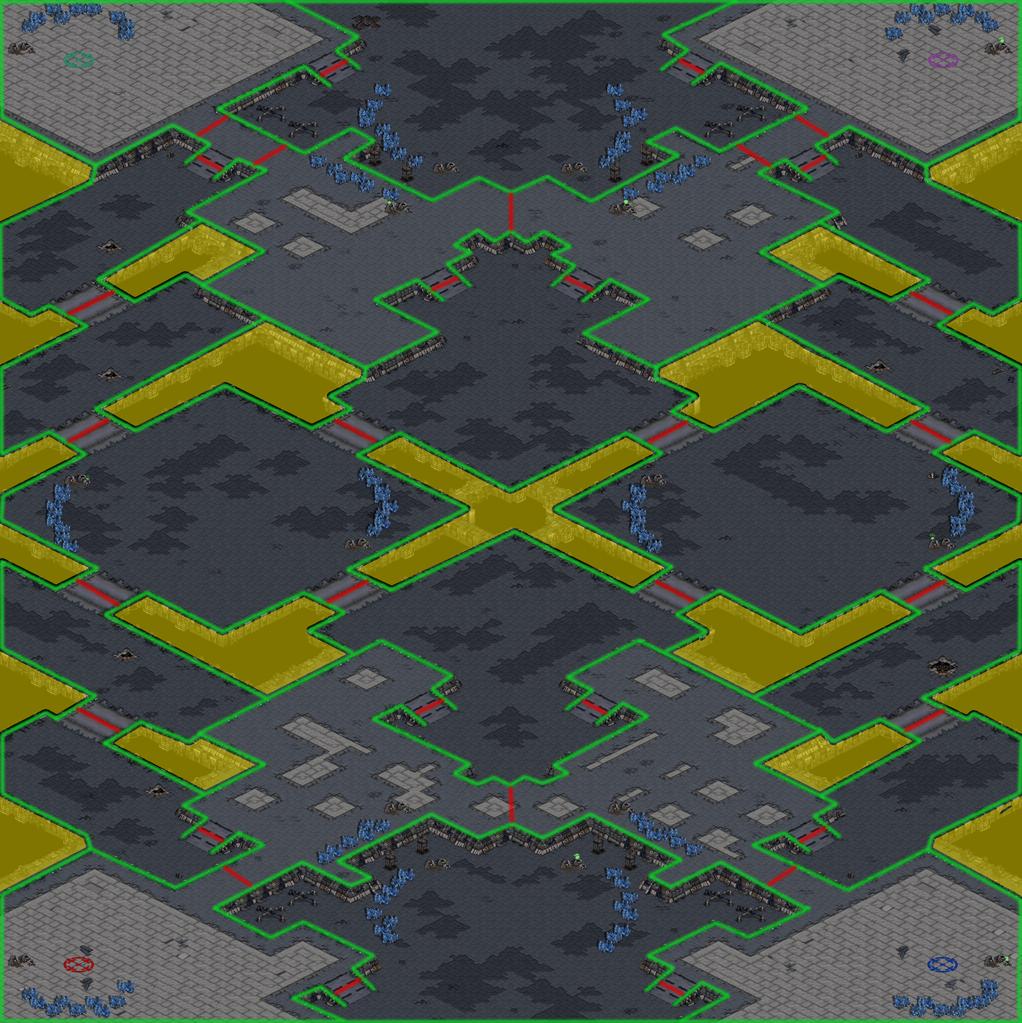
\includegraphics[width=0.8\textwidth]{space_atoll_(co-op)_regions_small}
	\caption[Regions and choke points]{Regions and choke points. \colorbox{green}{Regions} are surrounded by green lines, \colorbox{Red}{choke points} are denoted by a red line, and the yellow areas are \colorbox{yellow}{unwalkable terrain}.}
	\label{fig:region_and_choke_points}
\end{figure}
% !TEX root = ../../main.tex
% !TEX spellcheck = en_US
\section{Behavior and system overview}
In their article\cite{abraham10} Abraham and McGee mentions four teammate models.
\begin{description}
	\item[Master-slave model] The player commands the teammate bot fully, and the bot has little or
	  no artificial behavior.
	\item[Semi-autonomous slave model] The player commands the teammate bot when s/he desires. When
	  no command is active the bots behave autonomously. Although bots can behave autonomously they
	  will still always act as a slave.
	\item[Clone model] This requires that all teammate have equal abilities and roles; the main
	  reason is to complete the goal faster, i.e. the more teammates the faster it goes. E.g. almost
	  like fetching water 100 buckets of water from a distant well, you can manage it yourself but
	  it goes faster with more people.
	\item[“Buddy” model] Both player and bot has comparable weaknesses and the bot does not act just
	  as the player’s slave.
\end{description}
We would like to add another one, semi-autonomous model, which is how BATS works, i.e. acts
autonomously and it can take commands, but does not always listen to them, e.g. when BATS is under
attack and the teammate orders it to attack, BATS will rebel and ignore the command and instead stay
and defend its base; this means that BATS is not a slave (by their definition).

While the autonomous behavior of BATS is described throughout the rest of this chapter, an overview
will first be given.

The goal of BATS is to behave more like a human, i.e. use strategies that humans use, communicate
more like humans, and so forth, as it has been shown that at least enemy bots are more fun when they
behave like humans\cite{soni08}. \\
% TODO Find Yannakakis



Figure \ref{fig:system_overview} shows a high level overview of the most important classes of BATS.
The figure is a bit cluttered, but 7 of the 15 associations either go to the Squad or
IntentionWriter.

\begin{figure}[htb]
	\centering
	\begin{tikzpicture}[auto,node distance=3.8cm]
		\node [block] (player_army) {PlayerArmy\-Manager};
		\node [block, right of=player_army] (scout) {ScoutSquad};
		\node [block, right of=scout] (exploration) {Exploration\-Manager};
		\node [block, below of=player_army] (Commander) {Commander};
		\node [block, right of=Commander] (squad) {Squad};
		\node [block, right of=squad] (attack) {Attack\-Squad};
		\node [block, right of=attack] (attack_coordinator) {Attack\-Coordinator};
		\node [block, below of=Commander] (self_classifier) {Self\-Classifier};
		\node [block, below of=self_classifier] (build_planner) {Build\-Planner};
		\node [block, right of=build_planner] (defense) {Defense\-Manager};
		\node [block, right of=defense] (intention_writer) {Intention\-Writer};
		
		% Paths
		% From Commander
		\draw [uniDirectional] (Commander) -- (player_army);
		\draw [uniDirectional] (Commander) -- (squad);
		\draw [uniDirectional] (Commander) -- (intention_writer);
		\draw [uniDirectional] (Commander) -- (self_classifier);
		
		% From Defense manager
		\draw [uniDirectional] (defense) -- (squad);
		\draw [biDirectional] ([xshift=-0.5cm]defense.north) |- (self_classifier);
		\draw [uniDirectional] (defense) -- (intention_writer);
		
		% From squad
		%\draw [uniDirectional] ([xshift=0.5cm]squad.south) |- (5, -7.6) -| (intention_writer.north);
		
		% From scout
		\draw [inheritArrow] (scout) -- (squad);
		\draw [uniDirectional] (scout) -- (exploration);
		
		% From attack
		\draw [inheritArrow] (attack) -- (squad);
		\draw [biDirectional] (attack) -- (attack_coordinator);
		\draw [uniDirectional] (attack) -- (intention_writer);
		
		% From attack coordinator
		\draw [uniDirectional] (attack_coordinator) |- (exploration);
		\draw [uniDirectional] ([xshift=-0.5cm]attack_coordinator.north) |- (5,-1.9) -| ([xshift=0.5cm]player_army.south);
		
		% From Self classifier
		\draw [uniDirectional] (self_classifier) -- (build_planner);
	\end{tikzpicture}
	\caption{System overview of BATS}
	\label{fig:system_overview}
\end{figure}

The Commander is in charge of expanding, attacking, and scouting and uses SelfClassifier or
PlayerArmyManager to decide on what action it shall take—
PlayerArmyManager handles the teammate's
virtual squads and is used to see what the teammate does with those squads. Expansions can be created through
build orders, or added autonomously to the build order when BATS's resources are getting high. It
can also expand when it has launched an attack or vice versa, attack because it expands. Instead of
doing random attacks, it will try to create attacks when it expands, so the attack covers the
expansion which is a common (among professionals) and good strategy in StarCraft\cite{day9}. It can
also launch an attack if an upgrade will finish soon, or if the teammate is moving out to attack.
Scouting is done all the time, except the first couple of minutes in the game and when BATS is under
attack. Section \ref{sec:Commander} \nameref{sec:Commander} describes the triggers to expand,
attack, and scout in more detail.

DefenseManager decide where units (good at defending) shall be placed, i.e. close to choke points
that abuts to an undefended region. The rest of the units will patrol between the choke points. BATS
will however help the teammate player when s/he is under attack, but will never have any stationary
units there. Section \ref{sec:defense_manager} \nameref{sec:defense_manager} describes BATS's
defense in more detail.

Attack squads asks AttackCoordinator for a place to attack which prioritizes the location depending on the structure type and distance from other
attacks. It prioritizes important structures, such as newly created Expansions. The squad will
retreat when the enemy squad is too strong, or if it destroyed all structures near the attack
location. Section \ref{sec:attack_coordinator} \nameref{sec:attack_coordinator} further describes
where the Attack squads finds their location and \ref{sec:attack_squad} \nameref{sec:attack_squad}
describes Attack squads in more detail.

Scout squad moves to an location while trying to avoid enemies, the scout asks ExplorationManager
for the location to scout, which is the location that was visited the longest time ago. When it
either gets to the location or is interrupted by enemies it will ask for a new location to scout.

The Build planner creates structures from a build order, the build order is not fixed at
supply counts but is instead listed in order and the first (not built) structure in the build order
will be build directly when BATS has enough resources. BATS will, however, prioritize unit
production over all structures.

The Commander, DefenseManager, and AttackSquad uses IntentionWriter to
write messages; messages are sent by intention and an optional reason, the same intention will
however not be sent again if it is sent within the timeout limit.


% !TEX root = ../../main.tex
\section{Exploration manager}
\label{sec:exploration_manager}
The exploration manager in BATS have mostly gotten its functionality from BTHAI’s exploration manager, some functionality has been change, added, or removed to work better with BATS. The main functionality of the exploration manager is to keep track of when a region and expansion was last checked. It does this by by checking if either a region’s center or an expansion position is visible, if it is, it will automatically update the time of the last visit. This information is used by both \nameref{sec:scout_squad} to get the next scout location—i.e. the one with oldest visit time—and \nameref{sec:attack_coordinator} to get expansions that have not been visited for \attackCoordinatorExpansionNotCheckedTime—used for attacks. How \nameref{sec:scout_squad} and \nameref{sec:attack_coordinator} uses this functionality is described in section \ref{sec:scout_squad} and \ref{sec:attack_coordinator} respectively.

Exploration manager saves all buildings it has spotted, because BATS does not have full map vision and thus needs to save the information of the enemy. This is used by \nameref{sec:attack_coordinator} to get a all buildings to decide a place to attack and \nameref{sec:attack_squad} to find a common spot to attack when near the target location.
% !TEX root = ../../main.tex
% !TEX spellcheck = en_US
\section{Attack coordinator}
\label{sec:attack_coordinator}
Frontal attacks attack the enemy head on and usually use the majority of the player’s army,
distracting attacks are small attacks either used to distract the enemy from one position where
another attack will come (hence the name), or they can be used to try to deal some damage to the
enemy, with heavy emphasis on try. These distracting attacks can be drops, harassment,
counter-attacks\footnote{A drop when we are under attack can be called counter-attack, but our
meaning of counter-attack is a frontal attack, but smaller}—BATS has, in time of this writing, only
implemented the drop functionality. The distracting attacks are not suicide attacks, although
exceptions exist; they are mostly distractions to pin the enemy at his base.

\paragraph{Where to attack?} The attack coordinator uses two to three weights multiplied together to
get the near optimal attack location—the attack location is not optimal and that the weights have
not been extensively balanced, but the algorithm works good enough for these experiments. The
attacking locations are derived from seen enemy structures and expansions that have not been scouted
for \attackCoordinatorExpansionNotCheckedTime.

The first weight, \emph{distance}, prioritizes structures (and location) far away from other
existing attacks, not including allied attacks yet; as it is a good idea to spread out multiple
attack to split up the enemy army—i.e. we are not implying that multiple armies are better than a
big, only that when using multiple armies it is good for the armies to spread out. The second
weight, \emph{type}, determines how important a structure or location is to attack, and the third
weight, \emph{defended}, is how well defended an area is—the defended weight is not implemented yet,
but distracting attacks will use it to get a location that can be attacked without taking the risk
to die (such as drops dying to anti-air).

In addition to these weights, if the squad is a frontal attack and follows an allied squad, it will
get an attack position near the allied squads target instead of using the weights. The attack
position is still the same positions used for the regular algorithm.

Enemy armies are not included in the calculation, because one rarely gain anything on trading
armies, one should find gaps in the defense instead\cite{day9}. It is still good engage a weaker
enemy army and BATS will do that if the squad is close by, but it will not search for those small
armies. In addition, because armies are mobile it would be hard to track them, i.e. time consuming
to implement such a feature.

The flowchart in figure \ref{fig:AttackCoordinator::requestAttack()} shows an attack squad
requesting an attack from attack coordinator. It can either get an weighted attack location or join
the teammate's frontal attack, if s/he has one. Attack coordinator uses a rule based system to
decide the how and where the squad shall attack.
\begin{figure}[htb]
\centering
	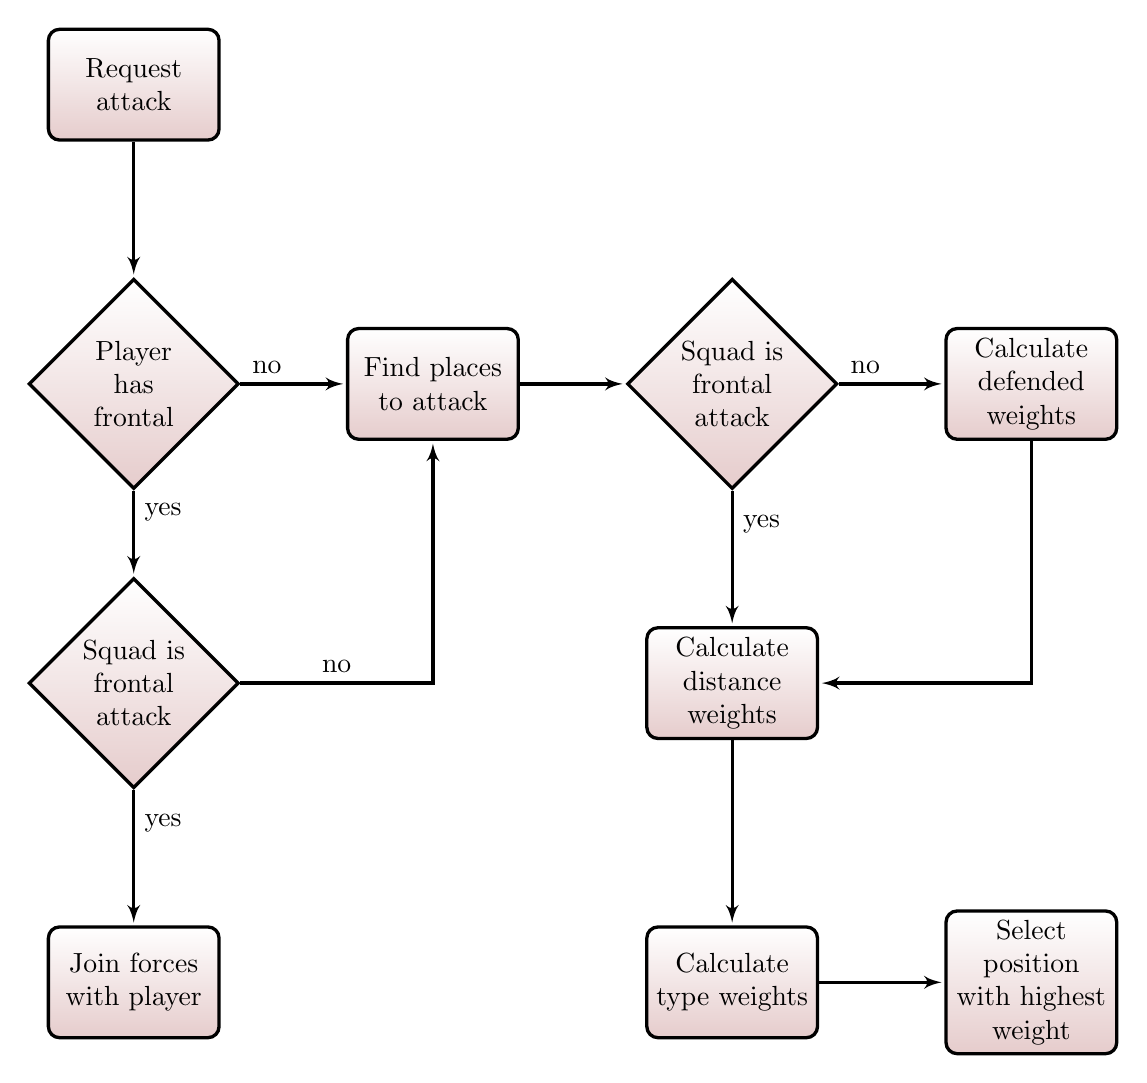
\begin{tikzpicture}[->,>=stealth,shorten >=1pt,auto,node distance=3.8cm]
		\node [block] (init) {Request attack};
		\node [decision, below of=init] (player_frontal) {Player has frontal};
		\node [block, right of=player_frontal] (find_places) {Find places to attack};
		\node [decision, right of=find_places] (bot_frontal) {Squad is frontal attack};
		\node [block, right of=bot_frontal] (defend) {Calculate defended weights};
		\node [decision, below of=player_frontal] (bot_frontal2) {Squad is frontal attack};
		\node [block, below of=bot_frontal2] (join_forces) {Join forces with player};
		\node [block, below of=bot_frontal] (distance) {Calculate distance weights};
		\node [block, below of=distance] (type) {Calculate type weights};
		\node [block, right of=type] (select) {Select position with highest weight};
		
		\path [line] (init) -- (player_frontal);
		\path [line] (player_frontal) -- node [near start] {no} (find_places);
		\path [line] (player_frontal) -- node [near start] {yes} (bot_frontal2);
		\path [line] (bot_frontal2) -- node [near start] {yes} (join_forces);
		\path [line] (bot_frontal2) -| node [near start] {no} (find_places);
		\path [line] (find_places) -- (bot_frontal);
		\path [line] (bot_frontal) -- node [near start] {no} (defend);
		\path [line] (bot_frontal) -- node [near start] {yes} (distance);
		\path [line] (defend) |- (distance);
		\path [line] (distance) -- (type);
		\path [line] (type) -- (select);
	\end{tikzpicture}
	\caption{Flowchart of Attack Coordinator’s requestAttack() function}
	\label{fig:AttackCoordinator::requestAttack()}
\end{figure}

\paragraph{Coordinated attacks}
To achieve a sense of coordinated attacks, attack squads have \nameref{sec:wait_goals} added by the attack coordinator—fully described in section \ref{sec:wait_goals}. The wait goal for attack squads is a wait goal that succeeds whenever an attack is within position (close to its goal and waiting), or is already attacking something. The goal fails when it has timed out (\attackCoordinatorWaitGoalTimeout). The wait goal is added to all existing squads and the new squad gets the already existing wait goals, when all attacks are in position they will start their attack simultaneously.

\subsection{Calculation of distance weight}
Distance weight is a simple calculation: if no other attack squads are present it defaults to 1.0. Otherwise the average from all other attacking squads are calculated as described in equation \ref{eq:distance_weight}.
\begin{equation}
\label{eq:distance_weight}
weight = \frac{\sum_{i=1}^{s}{distance(i)^2}}{s} \qquad \left\{s = \text{number of attack squads}\right.
\end{equation}
Here \emph{weight} is the average distance from all other attacking squads. The weight is then normalized to [0.0, 1.0], shown in equation \ref{eq:distance_weight_normalized}—dividing the weight with the maximum map distance. As with most distance calculations, they use the squared version for faster calculation since no root calculations are needed.
\begin{equation}
\label{eq:distance_weight_normalized}
normalized\ weight = \frac{weight}{MAP\_WIDTH^2 + MAP\_HEIGHT^2}
\end{equation}


\subsection{Calculation of type weight}
This weight prioritizes different structures and locations. Most of the values here are fixed and one type calculated between fixed values (expansions). The structures and locations are presented in priority order below with the current values assign to them. These values are rough estimates what might be good, thus one shall not think these are \emph{the} values. Because the weights are multiplied this will give a logarithmic behavior, i.e. the difference between 0.1 and 0.2 is greater than 0.2 and 0.3 (0.2 is the double of 0.1, whereas 0.3 is less than double of 0.2).

\paragraph{Not scouted expansions \attackCoordinatorWeightsExpansionNotChecked}
These are expansion that have not been visited for the last \attackCoordinatorExpansionNotCheckedTime. The idea is to check expansions when moving out to attack, although the current version does not work as expected; because the \nameref{sec:scout_squad} cannot cover all the areas quickly the attack squad will act more as a scout than attack squad because of visiting expansions in various location around the map. To fix this only the closest expansions to the enemy shall be checked and possibly only one with this squad, as this is roughly what Magnusson has observed when watching professional StarCraft players. This feature was therefore disabled during the experimentations.
	
\paragraph{Expansions \attackCoordinatorWeightsExpansionMinMax}
Expansion weight for existing enemy expansions. The weight is higher for fresh expansions; fresh expansions being defined by the expansions current mineral amount (in fractions)—the \nameref{sec:resource_counter} tracks the amount of all mineral fields.

The minimum value can, in addition to its normal state, be used as a kind of ceiling function; e.g. if it is set to ceil\conf and the minimum is set to 0.5 while only 20\% of the minerals are left it will ceil the weight to 0.5, see equation \ref{eq:weight_expansion_ceil}. If it is set to normal, the fraction will be normalized in the [0.5, 1.0] range, meaning the weight will be 0.6, see equation \ref{eq:weight_expansion_normal}.
\begin{equation}
\label{eq:weight_expansion_ceil}
weight =
\begin{cases}
minValue & if $fracMinerals(x) < minValue$ \\
fracMinerals(x) & if $fracMinerals(x) \geq minValue$
\end{cases}
\end{equation}
\begin{equation}
\label{eq:weight_expansion_normal}
weight = fracMinerals(x) \times (maxValue - minValue) + minValue
\end{equation}

\paragraph{Addons \attackCoordinatorWeightsAddonStructure}
Addons are structures built in connection to another structure and only exist for Terran. These are both upgrade structures and can make either the attached unit producing structure create advanced units (such as tanks), or all specific unit producing structures able to produce the unit—e.g. the addon Covert Ops for a Science Facility makes Ghosts available for production in all Barracks. The only exception to this is the addons to the Command Center which is either Comsat for detection or Nuclear Silo for nukes.

\paragraph{Supplies \attackCoordinatorWeightsSupplyStructure}
Supplies are structures that provide space (or food) for more units to be created, see section \ref{sec:starcraft_supply} for how supplies work. This supply priority only makes sense for Terran as they work differently for the other classes: Protoss also uses their supplies for powering buildings, i.e. a higher priority would be good here; for Zerg the supplies are increased by the Overlord unit, this would require an additional algorithm for searching for Overlords, the priority would be higher, maybe even higher for only air attacks.

\paragraph{Upgrade structures \attackCoordinatorWeightsUpgradeStructure}
Upgrade structures does not, despite its name, include all structures that can upgrade, only structures that can upgrade general attack and defense bonuses are treated as upgrade structures. Meaning Terran Academy (which upgrades Stim packs for Marines) is not treated as an upgrade structure. The reason is because of simplicity; attack and defense upgrades come in three steps meaning there are 6–12 upgrades in total (depending on what structure) for that structure and is continued to be upgraded throughout the game. This means its a lot bigger chance that the structure still is useful (for the enemy) even when attacking it later in the game, as opposed to the Academy which upgrades are long done—although in this case medics and firebats could not be created by the enemy, but the enemy can simply prioritize marines in the meanwhile and not much harm would be done.

As an improvement BATS could keep track of which upgrades it has seen and then exclude these buildings. Attack and defense upgrades can be directly seen on the enemy while unit abilities, but stim, and other ability upgrades needs to be activated by the enemy for BATS to know about it.

\paragraph{Unit producing structure \attackCoordinatorWeightsUnitProducingStructure}
All structures that can produce units. These are not ordered in any specific order, not to say that it does not matter because it does, but it will always vary depending on the situation. If the enemy has 10 barracks and 1 Starport, it is probably best to destroy the Starport, whereas if the enemy has 1 barrack and 4 Starports it might be best to destroy the barracks.

\paragraph{Other structures \attackCoordinatorWeightsOtherStructure}
All other structures that have not been covered, this includes research structures, but defensive
structures, such as bunkers and turrets.

\subsubsection{Why this order?}
Because StarCraft is mostly about managing expansions\cite{day9}, BATS tries to deny and kill fresh expansions as its first priority (the top two priorities). Targeting addons can both stop the production of an important upgrade (siege mode for tanks) and the ability to create tanks, ghosts, etc. Delaying late game units is usually good as they are generally better than early game units. Supply depots are almost always good to destroy since it halts all unit production, unless the enemy has stacked up lots of supplies—which almost always is a bad strategy—or lost many units in a recent battle. Stopping an upgrade is probably better than killing a unit producing structure, because if the upgrade finishes all existing units will get the upgrade, while if we kill a unit producing structure only 2–4 units will get stopped, but it depends on the type of unit producing structure, what upgrade structure etc; but this priority will do for now.

% !TEX root = ../../main.tex
% !TEX spellcheck = en_US
\section{Commander}
The Commander creates all orders for BATS, except defenses as the \nameref{sec:defense_manager} does that. This means that it orders attacks, drops, expansions, scouts, and when to transition to the next phase.

\subsection{Orders/Commands}
Below all orders are described and how they work depending on the current state of BATS. In addition some orders can have a slightly different behavior depending if it was BATS or the teammate who ordered it. Because of all tests and different behaviors in the command these are described with mostly pseudo-code. Common for all order functions are the two parameters: \texttt{alliedOrdered} and \texttt{reason}; alliedOrdered is set to true if the teammate ordered the command, reason is the reason to print out if the command is successful, this is only used when BATS ordered the command—e.g. expand because BATS expands.

\paragraph{Attack}
Has in general three behaviors: Creates a new frontal attack, reinforces the existing frontal attack, or does nothing.
\begin{lstlisting}[label={lst:order_attack},caption={Pseudo-code of the attack command}]
// Never do a frontal attack when under attack
if (isUnderAttack()) {
	if (alliedOrdered) {
		mIntentionWriter->write(BotAttackNot, BotIsUnderAttack);
	}
	return;
}

// Teammates can create attacks even if few units
if (alliedOrdered) {
	canAttack = !freeUnits.empty();
} else {
	canAttack = canFrontalAttack(); // Checks enough units
}

if (canAttack) {
	oldSquad = mSquadManager->getFrontalAttack();
	
	// Add free units to the old attack squad if it exists
	if (oldSquad != NULL) {
		oldSquad->addUnts(freeUnits);
		mIntentionWriter->write(BotAttackMerged, reason);
	}
	// Create new attack and ping position
	else {
		attackSquad = newAttackSquad(freeUnits);
		attackPos = attackSquad->getAttackPosition();
		mIntentionWriter->write(BotAttack, reason, attackPos);
	}
} else {
	mIntentionWriter->write(BotAttackNot, BotNotEnoughUnits);
}
\end{lstlisting}

\paragraph{Follow}

\paragraph{Drop}

\paragraph{Scout}

\paragraph{Expand}

\paragraph{Transition}

\subsection{Order creation rules}
The Commander can create orders either from its own actions and states, or what the allied player is doing. Examples of this is it might attack when it is expanding, and it might expand if it has high amount of minerals, for reaction to allied actions it attack if the allied player is expanding.

\subsubsection{Reacting on own actions and states}
The commands are ordered by commands in own reactions.

\paragraph{Expand}
In order to expand from own reactions BATS meet all conditions below.
\begin{enumerate}
	\item Not be under attack—expanding when we are under attack will most likely kill the expansion directly
	\item Not already be expanding—we do not want to spam expansions
	\item Active expansion count needs to be less than \commanderExpansionActiveMax—good number of active bases as it keeps a large and steady income to support many unit producing structures. Active expansions are expansions where at least \classificationExpansionExpansionMineralsLow~minerals left.
	\item No new expansion should have been build in \commanderExpansionIntervalMin, again we do not want to spam expansions and this seemed like a reasonable time, but has not been extensively tested.
\end{enumerate}
When all four conditions are met it will check if any of the following conditions are met, if they are an expansion will be added to the beginning of the build order.
\begin{enumerate}
	\item BATS has an attack—good idea to expand when attacking (or vice versa), distracts the enemy from the expansion long enough for the expansion to complete\cite{day9}.
	\item Expansions are saturated—generic expansion rule to expand when low on expansions, i.e. below max active expansion count. Expansions are saturated tests if the number of workers per mineral patch (thus per expansion) is at or above \classificationExpansionWorkersPerMineralSaturation !!! CITE !!!\marginpar{CITE}. % Cite workers per mineral saturation from team liquid
	\item An expansion is running low on minerals—making sure we stay on the same number of active expansions. This is the same as an expansion that is not active (i.e. having less than \classificationExpansionExpansionMineralsLow~minerals left) but still having some minerals left to be mined.
	\item High on minerals—if we have too much minerals that means we cannot build enough structures or units, thus we can as well add another base and possibly increasing the amount of gas mined. Activates when the mineral count is above \classificationHighOnMinerals.
\end{enumerate}

\paragraph{Attack}
To attack from own reactions BATS shall meet all conditions below.
\begin{enumerate}
	\item Shall not be under attack—it is better to stay and defend and then possibly attack, although a small counter attack might be effective when the enemy army is small and BATS can spare some units for the attack, this functionality has not been implemented.
	\item Not have a current attack—having one big army is easier to control and generally much stronger than splitting it into 2 smaller attacks for slower armies\cite{day9} as BATS will use in the experiment. Although ordering a second attack when we have a frontal attack will reinforce units, but we did not have enough time to implement and test when to reinforce the army.
\end{enumerate}
When all two conditions are met it will check if any of the following conditions are met, if they are an attack will be created.
\begin{enumerate}
	\item Expanding—as explained earlier under the expand, it is good to attack while expanding.
	\item Upgrade soon done—when an upgrade will finish soon this means that the bot will get stronger and it might be possible that the enemy has either not caught up in upgrades, i.e. the longer we wait the less valuable the upgrade is\cite{day9}. Upgrade soon done checks if any of the free units that could be used for an attack will be affected with an upgrade that is currently upgrading and if the upgrade finishes within \classificationUpgradeSoonDone.
\end{enumerate}

\paragraph{Scout}
The scout order conditions are much simpler than expand and attack. BATS will always send out a scout if it it is not scouting, not under attack and has \commanderScoutOnWorkerCount.

\paragraph{Transition}
The transition order conditions are just as simple as the scout. IT will transition if it is not already in late game, no buildings in the build order, and is high on resources. It is high on resources when both the mineral and gas count is higher or equal to \classificationHighOnMinerals~and \classificationHighOnGas~respectively.

\subsubsection{Reacting on allied actions}
All orders here are grouped by allied actions instead of the commands (as reacting on own actions were), this feels like a more intuitive approach and was implemented this way.

\paragraph{Allied expands}
If the allied player expands, BATS first want to create a distracting attack (for now only drops are available) to distract the enemy from the expansion, if no drops are available it will create a frontal attack. But before the commander creates any attack it checks so that we are not under attack or already attacking.

\paragraph{Allied attacks}
Depending on what type of attack the allied player has BATS behaves differently, but common for all types of attack, it will not do anything if it is under attack. If the allied attacks with a frontal attack BATS will first try to join it, if it already does not have a frontal attack and has enough units (\classificationFrontalAttackUnitsMin) for a frontal attack, otherwise it will try to drop if it does not have a drop out and has enough units for a drop.

When the allied player has a distracting attack out BATS will too try to create a distracting (drop) attack, but will only succeed if it has enough units.

% !TEX root = ../../main.tex
% !TEX spellcheck = en_US
\section{Defense manager}
\label{sec:defense_manager}
The defense manager handles the defense of both defending its own base and the player’s base. It calculates defense locations and where \nameref{sec:hold_squad}s shall be placed and between which positions the \nameref{sec:patrol_squad} patrols.

The defense locations are calculated from choke points that abut either BATS’s or the allied’s currently occupied regions. It does not defend choke points to empty regions where this region only abuts to BATS or allied occupied region, this can be seen in figure \ref{fig:defense_locations} where the empty region is outlined in green.

The defense locations are defended by \nameref{sec:hold_squad}s and a \nameref{sec:patrol_squad}. The hold squads, described fully in section \ref{sec:hold_squad}, are stationary and defend the choke point from a certain roaming perimeter, where the center is calculated by finding a position in the range \squadDefendRoamDistanceMinMax~closest to one of BATS’s or the allied’s buildings and the radius being \squadDefendRoamPerimeter. Units from the hold squad will stay in the roaming perimeter until enemy units enter the defense perimeter (\squadDefendDefendPerimeter~in radius), they will then start to attack the enemy. 

Figure \ref{fig:defense_locations} displays an example of where Defend locations can be, how regions are interpreted, and so forth.

%: Add picture with locations that are defended, including roam positions
\marginpar{Add picture with defend locations}
\begin{figure}[htb]
\centering
\caption{Example of defense locations. Green outlined regions are BATS’s regions, blue outlines are allied’s regions, regions outlined with both green and blue belong to both. Yellow regions are non-defended as they abut only BATS or allied regions. Defense locations are outlined with}
\label{fig:defense_locations}
\end{figure}

Patrol squads on the other hand contains all free units, these will patrol between the defense locations. If enemy units enter the enemy offensive perimeter (\squadDefendEnemyOffensivePerimeter~in radius) in a defense location all squad units will move to the defend location to defend it, all other hold squads will disband to join the defense in the patrol squad. The idea was first to only disband the other hold squads if the enemy is too strong, but the calculation proved difficult and we focused work on other more improtant areas. This strategy was tested and it works good against one StarCraft default AI, as it only attacks from one location at a time. Two default AIs can however attack from different locations, but usually attacked from one location, but was in general too strong for BATS to defend by itself. Although it worked against the default AI it would not work against other AIs or humans that can attack two different locations simultaneously.


Both hold squads and patrol squads roam or patrol between BATS’s defense location so the bot won’t disturb the allied player with its units.

\paragraph{Defending other locations}
Although no hold squads are located on and the patrol squad never patrols on the teammates defend locations. It will still send the patrol squad to defend a teammate defend locations if BATS is not under attack itself. In addition to defending all defend locations, the defense manager will send out the patrol squad to defend locations either inside BATS’s or the teammate's base that are under attack, for example if the enemy drops inside the base. This will, however, never bring the hold squads as they should defend the entrance to the base.
% !TEX root = ../../main.tex
% !TEX spellcheck = en_US
\section{Player classification}
The player classification is split into two separate modules. One handles the grouping of teammate
and enemy virtual squads. They are virtual as these are BATS estimations that they belong to the
same squad. The other module groups common classifying tests for both teammate and BATS. 

\subsection{Player squads}
The \texttt{PlayerArmyManager} creates and holds all the virtual squads, both teammate and enemy
squads. Teammate and enemy squads derive from the PlayerSquad class which keeps a record of its own
center position and supply count for the last \classificationMeasureTimeTotal; this enables more
complex calculations, such as the direction of the squad and if it's increasing/decreasing in size.
These are the most important PlayerSquad function:
\begin{function_description}
	\item[\texttt{TilePosition getCenter()}] Current center position of the squad.
	\item[\texttt{int getDeltaSupplyCount()}] How many supplies have increased or decreased during the
		last \classificationMeasureTimeTotal.
	\item[\texttt{TilePosition getDirection()}] Non-normalized direction between the center of the
		squad during the last \classificationMeasureTimeTotal.
	\item[\texttt{int getSupplyCount()}] Current supply count.
	\item[\texttt{TilePosition getTargetPosition()}] Calculates where the majority of the units has as
		a target position. Useful when wanting to know where the player is heading.
	\item[\texttt{int getUnitCount()}] Number of units in the squad.	
\end{function_description}

\paragraph{Grouping algorithm}
Simply put, player army manager starts creating a virtual squad for a teammate player and then
searches for close units within the include distance (\classificationSquadIncludeDistance) to
include in the squad. The next update it will start with a unit already in a squad and again try to
include new units, but it will also remove units from the squad that are further away than the
exclude distance (\classificationSquadExcludeDistance). Enemy squads are created the same way as
teammate squads.

Testing the distance between so many units were too computational heavy, even when using the squared
distance version with no square roots. Instead units are inserted in a grid with a width of half the
exclude distance. Using half the exclude distance decreased the number of distance computations
further. Figure \ref{fig:player_squad_group_grid} shown an example of the grid with outlined include
and exclude distances. To further increase the computation speed, instead of computing which grid
the unit shall be placed in a lookup table is used instead.

\begin{figure}[htb]
\centering
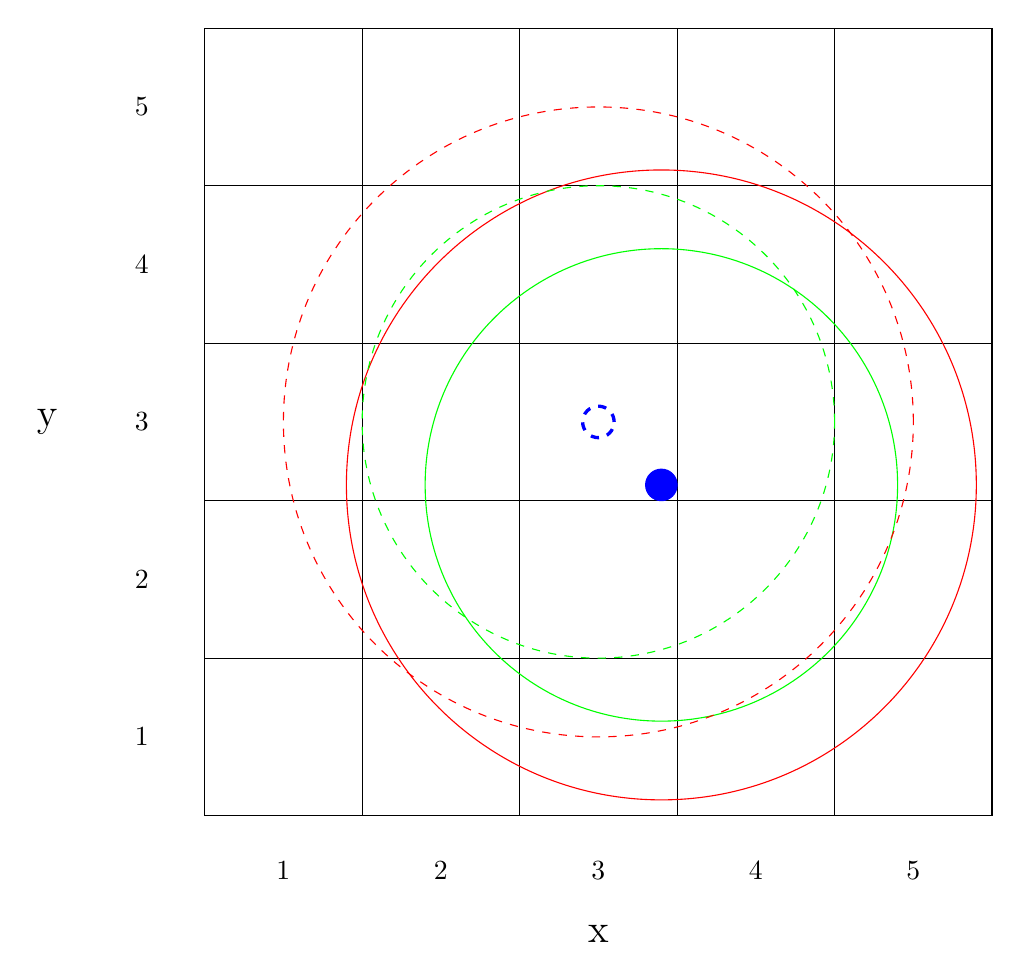
\begin{tikzpicture}[scale=2]
	% grid lines
	\draw (0, 0) grid (5, 5);

	% text coordinates
	\node at (-1, 2.5) {\Large{y}};
	\node at (2.5, -0.75) {\Large{x}};

	% coordinate values
	\foreach \i in {1,...,5} {
		\node at (\i-0.5, -0.35) {\i};
		\node at (-0.4, \i-0.5) {\i};
	}

	% filled unit
	\filldraw[blue] (2.9, 2.1) circle(0.1);
	\draw[red] (2.9, 2.1) circle(2);
	\draw[green] (2.9, 2.1) circle(1.5);

	% second dashed unit
	\draw[blue,very thick,dashed] (2.5, 2.5) circle(0.1);
	\draw[red,dashed] (2.5, 2.5) circle(2);
	\draw[green,dashed] (2.5, 2.5) circle(1.5);
\end{tikzpicture}
\caption[Minimizing distance calculation using grids]{
	Example of using grid to minimize distance calculations.
	\usebox{\LegendDotBlue} The unit.
	\usebox{\LegendCircleGreen} include distance;
	\usebox{\LegendCircleRed} exclude distance.
	The dashed circles represents another unit, its include and exclude distances from the middle of a grid square.}
\label{fig:player_squad_group_grid}
\end{figure}

\begin{lstlisting}[label={lst:player_squad_rearrange_squads},caption={Pseudo-code of \texttt{rearrangeSquads()}}]
// Iterate through all squads, one unit each turn
do {
	foundUnit = false;
	while (moreUnitsToCheck() && !foundUnit) {
		if (unitSquad.isValid() && !squadChecked(unitSquad) {
			currentUnit = unit;
			foundUnit = true;
		}
	}
	
	if (foundUnit) {
		setUnitAsChecked(currentUnit);
		setSquadAsChecked(unitSquad);
		
		addCloseUnitsToSquad(currentUnit, unitSquad.getId());
	}
} while (foundUnit);

// Create new squads for the rest of the units that either
// went outside the squad's bounds or never had a squad
while (moreUnitsToCheck()) {
	setUnitAsChecked(unit);
	newSquad = new PlayerSquad();
	setSquadAsChecked(newSquad);
	addCloseUnitsToSquad(unit, newSquad.getId());
}
\end{lstlisting}

Only units within two grid units are used when calculating the distance, this generates a 5x5 grid
just as figure \ref{fig:player_squad_group_grid}. As can be seen in the figure units further away
than two grid units can never be within the exclude distance. Units in the same grid or to the left,
top, right, or bottom are almost always within the exclude distance, an exception can be seen in the
figure where small portion of the upper left corner at (2,3) is outside the solid exclude circle;
for simplicity all units within these grid positions are seen as within the exclude distance (even
though exceptions might exist).

To make use of these calculation benefits, units in a squad are checked first (if they are further
away than the exclude distance). A simplified pseudo-code example is shown in listing
\ref{lst:player_squad_rearrange_squads} where high-level calculations are made and in listing
\ref{lst:player_squad_add_close_units_to_squad} where calculations of close units to add to the
squad—note that units are not excluded form the squad here, they are not excluded until they are
added in another squad which happens at the end of \texttt{rearrangeSquads()}.

\clearpage

\begin{lstlisting}[label={lst:player_squad_add_close_units_to_squad},caption={Pseudo-code of \texttt{addCloseUnitsToSquad()}}]
// Add all units that are in the same square or the
// bordering left, top, right, bottom square.
foreach (square in same, or border square) {
	foreach (not checked unit in this square) {
		if (same squads as paramUnit) {
			queuedUnits.push_back(unit);
			setUnitAsChecked(unit);
		} else if (withinIncludeDistance(unit, paramUnit) {
			queuedUnits.push_back(unit);
			setUnitAsChecked(unit);
		}
	}
}

// Recursively check queued units, this is done afterwards so
// that all fast calculations can be done first
while (!queuedUnits.empty()) {
	addCloseUnitsToSquad(queuedUnits.front(), squadId);
	queuedUnits.pop_front();
}

// Directly recursive, instead of queueing units it will directly
// call addCloseUnits... because those units could add close units
// that were within bordering squares that otherwise would be
// calculated here using distance calculations.
// Uses the full 5x5 square, except squares already checked
foreach (other square) {
	foreach (not checked unit in this square) {
		if (same squad as paramUnit) {
			if (isWithinExcludeDistance(unit, paramUnit) {
				setUnitAsChecked(unit);
				addCloseUnitsToSquad(unit, squadId);
			}
		} else if (isWithinIncludeDistance(unit, paramUnit) {
			setUnitAsChecked(unit);
			addCloseUnitsToSquad(unit, squadId);
		}
	}
}
\end{lstlisting}


\subsection{Grouped classifying tests}
A common class uses the facade pattern to group both easy and complicated tests into one class to
minimize the coupling between classes, reuse code, and have to have the code in one place if a tests
was to change (instead of changing it in several places)—e.g. a simple test like
\texttt{canFrontalAttack(units)} which returns true if the unit size is larger or equal to the
minimum number of units BATS needs for a frontal attack:
% \vspace{-1.5em}
{\center{\texttt{\justify return units.size() >= FRONTAL\_ATTACK\_UNITS\_MIN;}}\\}
\vspace{0.5em}
None of the classifying classes modifies any data, thus all functions
are const and all three classes (although an enemy classification was not implemented) were supposed to have a
common interface to make it easier to use all three classes without having to learn three different
interfaces. Due to lack of time and not being the most important aspect this feature was skipped in
this version.

\paragraph{Self classification}
This classifier groups together common tests for BATS and might not be seen as a classifier.
\nameref{sec:commander} and \nameref{sec:defense_manager} uses the self classifier to easier
calculate their goals and decrease their coupling. Below all important functions are listed and
described, although most of the names should be self-explanatory.

\begin{function_description}
	\item[\texttt{bool areExpansionsSaturated()}] Tests if there exists enough workers to saturate all mineral patches.
	\item[\texttt{bool canDrop()}] If BATS have enough units to create a drop.
	\item[\texttt{bool canFrontalAttack()}] If BATS have enough free units to create an attack. This is only used for when BATS want to create an attack, if the teammate orders an attack it is enough with one unit.
	\item[\texttt{int getActiveExpansionCount()}] Number of active expansions, i.e. expansions with more than \classificationExpansionExpansionMineralsLow.
	\item[\texttt{double getLastExpansionStartTime()}] How many game seconds ago the last expansion was started.
	\item[\texttt{bool hasDrop()}] Checks if BATS has a drop.
	\item[\texttt{bool isAnExpansionLowOnMinerals()}] Checks if an expansion has less than \classificationExpansionExpansionMineralsLow.
	\item[\texttt{bool isAttacking()}] Checks if we have an attack squads that is not retreating.
	\item[\texttt{bool isExpanding()}] Checks if BATS is either expanding or going to expand (expansions in build order).
	\item[\texttt{bool isHighOnGas()}] BATS has more than \classificationHighOnGas~gas.
	\item[\texttt{bool isHighOnMinerals()}] BATS has more than \classificationHighOnMinerals~minerals.
	\item[\texttt{bool isScouting()}] If BATS has a scout squad out.
	\item[\texttt{bool isUnderAttack()}] Checks if BATS is under attack, uses Defense Manager's isUnderAttack().
	\item[\texttt{bool isUpgradeSoonDone(affectedUnits)}] Checks if an upgrade, that will affect the specified units, completes within \classificationUpgradeSoonDone.
\end{function_description}

\paragraph{Teammate classification}
The teammate classification works just as the self classifier described above, but at the moment only has one function, isExpanding(), as the squad functionality was implemented in PlayerArmyManager. isExpanding() checks if the teammate currently constructs a new base structure (e.g. Command Center).

% !TEX root = ../../main.tex
% !TEX spellcheck = en_US
\section{Squads}
A squad, in BATS, are units grouped together acting in coordination. All squads have the abstract Squad class as their base class. 

\paragraph{Creating, deleting, and retrieving squads}
The squad manager updates and removing existing squads (but only from the squad manager); any class can create a squad and it adds itself automatically to the squad manager (via the squad's constructor). The squads are added as \texttt{shared\_ptr}, meaning they are automatically destroyed when no more references exist, i.e. no memory leaks. When a squad holds no units—achieved when all units died, units moved to another squad, or the squad disbands—the squad manager automatically removes it; but it can still be used if another class saved it before it was removed. Removed Squads have to be recreated to be inserted into the squad manager again.

Squads can be retrieved using two (actually four) different functions, either by the squad's id (automatically set) or by squad type (template function), shown in listing \ref{lst:SquadManager::getSquads()}. The template function will also return all sub-classes to the specified class, meaning \texttt{getSquads<AttackSquad>();} would return both attack squads and drop squads because drop squad derives form attack squad. The last two functions are there for convenience, the first returns the current frontal attack (if one exist), and the other returns all distracting attacks.
\begin{lstlisting}[caption={Template function to retrieve squads of the specified type},label={lst:SquadManager::getSquads()}]
template <typename T>
vector<shared_ptr<T>> SquadManager::getSquads();
\end{lstlisting}

\subsection{Squad base class}
Only the core functions of the squad base class are covered below, as there are too many helper functions to cover them all. If the reader wants to find out more information about the internal structure of the squads, s/he can look in Appendix \ref{sec:doxygen}. Squad movement will be covered first, then the squad's basic behaviors, which can be overridden by derived classes; and finally how the \texttt{update()} and \texttt{updateDerived()} functions work.

\paragraph{Squad movement}
This is not the specific unit movement, but where the squad's units move to. The potential field manager takes care of how units move and was already implemented in BTHAI\cite{bthai}—although some minor changes have been made to the potential field manager to accept some general squad behavior, more specifically moving towards the retreat location when retreating and when close to enemies. The squad has five prioritized locations it can move to. Starting from the lowest priority is
\begin{enumerate}
	\item The goal location where the squad want to go to do their main task (e.g. scout, attack, defend location).
	\item A retreat location to be able to retreat from e.g. an attack; there is no automatic retreat behavior in the base class, derived squads has to set the retreat location and the base class calls \texttt{onRetreatCompleted()} when the retreat succeeds or fails.
	\item To move to either the goal or retreat location a via path, that holds with multiple locations, can be used. Useful when attacking or retreating with a drop to make it move along the map's edges so that it does not run straight through the enemy.
	\item Temporary goal location, used when derived classes need an additional goal location, such as \nameref{sec:attack_squad}s waiting in a location to attack or \nameref{sec:hold_squad}s moving from their roaming area to the defended area when an enemy enters the defend perimeter. The temporary goal location is, however, disabled when a retreat location is active.
	\item Regroup location, the regroup is automatically handled by the squad when units are too spread out—a unit is further away than \squadRegroupDistanceBegin from the squad's center, the regroup stops again when all units are within \squadRegroupDistanceEnd. The squad will regroup to the unit who is closest to the goal position—first the squad's center was used but this caused units in the front to move backward and did not work very well, in addition the squad movement felt weird as if BATS could not decide what it wanted. Bugs can still occur when moving around a C shaped cliff as units to the left of the C are further away then those at the bottom location, if the goal is to the right of C. The regroup functionality can be disabled by derived classes, useful when sending reinforcements to the squad.
\end{enumerate}

\paragraph{Behaviors}
The squad has four elements that can change the behavior of the squad.
\begin{description}
	\item[Regrouping] which has been fully described above in squad movement.
	\item[Retreating]. While the base class squad never uses this directly, derived classes can set a retreat location and the squad will then check when it is close to the retreat location. Once close it will call \texttt{onRetreatCompleted()} which has the default behavior of disbanding the squad, thus merging it with the Patrol squad. By overriding this function another behavior can be accomplished. Retreat locations are most commonly retrieved from \nameref{sec:defense_manager} via the \texttt{findRetreatPosition()}, if a squad uses another location this will be mentioned.
	\item[Unit composition] a unit composition limits the squad to only contain units of the specific type, useful when creating special type of squads. Section \ref{sec:unit_composition} describes unit composition in more detail.
	\item[Avoid enemies] Some squads do not want to get close to enemies, in this case avoid enemies can be turned on. This causes attacking units to move to a specific location without attacking while trying to avoid enemies, this works most of the time but not always; the potential field manager in BTHAI did not support this behavior entirely as it needs to check that the unit retreats in the right direction, this was slightly improved by adding the goal location to the potential field calculation when avoid enemies is set, the calculation of goal location was already implemented but not used in BTHAI.
	\item[Wait goals] has been mentioned earlier in section \ref{sec:attack_coordinator} \nameref{sec:attack_coordinator} and is fully described in section \ref{sec:wait_goals} \nameref{sec:wait_goals}. While adding these does not give the base squad any specific behavior, they can be used in the derived classes for trigger behaviors.
\end{description}

\subsection{Attack squad}
\label{sec:attack_squad} The attack squad can both function on its own, but is also the base class
for all attacks—in the current version only drops derives attack squad. Used alone, it can either do
a regular attack or follow a teammate squad—a regular attack or battle in this section is a synonym
for an attack or battle where it not follows a teammate squad.

For regular attacks the squad requests an attack from \nameref{sec:attack_coordinator} to get an
attack location to move to and regroup when needed. When the squad is close to the attack location
(\squadAttackWaitingPositionDistanceFromGoal), i.e. its wait location, it will wait here until all
its wait goals are finished, then it will continue moving to its attack goal. This will sync the
attack with other attacking squads as they wait until the squad either is in the wait location,
under attack, or already attacking.

If it encounters any enemies on the road it will try to kill them, unless they are too strong where
the squad will retreat instead; the squad can decide to retreat from any regular battle at any time,
depending on the situation. For an attack to succeed with its mission all structures within the
radius of \squadAttackStructuresDestroyedGoalDistance from the attack location needs to be
destroyed. After succeeding with the mission the squad will retreat back to the base, disband the
squad, and merge with the \nameref{sec:patrol_squad}.

\paragraph{Following a teammate squad}
To follow a teammate squad it can either be set directly when creating the attack squad or later by
a call to \texttt{followTeammateSquad(teammateSquad)}, this converts the regular attack to follow
the specified squad—attack squads can only convert to following a teammate and not from.


\begin{lstlisting}[caption={Squad actions depending on the teammate squad's state},label={lst:attack_follow_allied}]
switch (mTeammateSquad->getState()) {
	// Regroup if not close
	case IdleOutsideBase:
		handleTeammateRegrouping();
		setAvoidEnemyUnits(true);
		break;
	
	// Go to teammate target location, don't attack
	case Retreating:
		if (isRegroupingWithTeammate()) {
			clearTeammateRegrouping();
		}
		setGoalPosition(mTeammateSquad->getTargetPosition());
		setAvoidEnemyUnits(true);
		break;

	// Go to target location, attack if see anything
	case MovingToAttack: 
		if (isRegroupingWithTeammate()) {
			clearTeammateRegrouping();
		}
		setGoalPosition(mTeammateSquad->getTargetPosition());
		setAvoidEnemyUnits(false);
		break;

	// Find something close to attack
	case Attacking:
		handleTeammateRegrouping();
		if (!isRegroupingWithTeammate()) {
			setAvoidEnemies(false);
			msAttackCoordinator->requestAttack(this);
		}
		break;

	// Retreat, then merge with Patrol Squad (disband)
	case IdleInBase:
		setRetreatPosition(mpsDefenseManager->findRetreatPosition());
		mTeammateSquad.reset();
		break;
}
\end{lstlisting}
When the squad follows an teammate squad it behaves differently, depending on the teammate squad's
current state, described below in listing \ref{lst:attack_follow_allied}.

While most of the code speaks for itself, some functions need extra clarification.
\texttt{handleTeammateRegrouping()} checks if the distance to the teammate squad becomes to large
(\squadAttackAlliedRegroupBegin), it both sets the regrouping location to the teammate's center
location and the squad to avoid enemy units—the regrouping is considered done when the distance
between the squads are less or equal to \squadAttackAlliedRegroupEnd~away.
\texttt{setGoalPosition(mTeammateSquad->getTargetPosition())} sets the squad to move to the location
where most of the teammate squad's units are moving to; thus it will meet up with the teammate's
squad around that location. If handleTeammateRegrouping() was used it would try to chase after the
squads current location—much like in football (soccer) you shall run where the ball is heading and
not where its current location. This also allows the teammate to control where the bot shall attack
as it will attack where the player decides to attack.

\texttt{mpsAttackCoordinator->requestAttack(this)} uses \nameref{sec:attack_coordinator} to find a place to attack; as mentioned in section \ref{sec:attack_coordinator} it will find an attack location close to the teammate squad's target. Why not use the target as with MovingToAttack and have the AttackSquad create the attack location? Because
\begin{inparaenum}[1\upshape)]
	\item we want all attack request to be in the same location, if the attacks needs to be fixed or better coordinated we only need to change it in one place;
	\item in the future the squad could get a location of a prioritized building to attack; and
	\item using teammate target directly it will cause our units to fight exactly where the player is, which might crowd the place not making all units able to fight, but could be better if squads are smaller—more experimentation on this subject is needed.
\end{inparaenum}

In addition the squad need to cope with when the teammate squad splits or merges with another teammate squad. If the current teammate squad is empty of units (as it can become when it merges with another teammate squad) it will search for close (\squadAttackFindAlliedSquadDistance) teammate squads and follow the largest squad. If no teammate squads were found, it will retreat and then disband.

\subsection{Drop squad}
\label{sec:drop_squad}
A drop squad is an attack containing a flying transportations along with some offensive units it
carries. The goal of the drop is to attack the enemy base from an undefended angle (as flying units
can fly over all terrain). In ideal situations the drop will unload its units and destroy either
significant bases or workers, but the goal is rather to distract the enemy for various reasons—e.g.
expanding and we do not want the enemy to attack, or the dropping player will attack from another
location simultaneously.

The drop squad uses attack squad as its base class. Listing \ref{lst:drop_squad} shows the behavior of the squad.

\clearpage
\begin{lstlisting}[caption={Drop squad behavior},label={lst:drop_squad}]
switch(mState) {
case LoadUnits:
	if (isTransportDoneLoading()) {
		setState(Transport);
	}
	// Note, no break!

case Transport:
	// travelsByGround() = cannot load all units
	if (travelsByGround() && !isRetreating()) {
		setState(Attack);
	} else if (isEnemyAttackUnitsWithinSight()) {
		if (isEnemyFasterThanTransport()) {
			setState(Attack);
	} else {
		if (!hasWaitGoals() && isTransportInGoalRegion()) {
			setState(Attack);
		}
	}
	break;

case Attack:
	// If we cannot load all units, don't load
	if (travelsByGround()) {
		break;
	}

	// Retreat when enemy units arrive, unless they are faster than us
	if (isEnemyAttackUnitsWithingSight()) {
		if (!isEnemyFasterThanTransport()) {
			setState(LoadUnits);
		}
	}
	// No enemies within sight, load if we aren't in the goal region
	else {
		if (!isTransportInGoalRegion()) {
			setState(LoadUnits);
		}
	}
	break;
}
\end{lstlisting}
While the code explains it self, setState() does not, as it changes the behavior of the squad. \texttt{setState(LoadUnits)} loads all ground units and disables regrouping; \texttt{setState(Transport)} enables regrouping again; and \texttt{setState(Attack)} sets the transportation to unload all units and enables regrouping.

The drop squad uses the same method as attack squad to check if its goal has completed, although it rarely does. Because the goal of the drop is not to destroy all buildings, merely to distract the enemy, it also has a timeout function which will make the drop retreat after \squadDropAttackTimeout, but only if it's not currently in the target region.

Now you know how it works, but which units will be used for the drop, as drops should not just use
random units and hope for the best? It uses \nameref{sec:unit_composition}s for this—section
\ref{sec:unit_composition} describes the unit composition and the drop's unit compositions, i.e. all
available squads, can be found in listing \ref{lst:unit_comp_drop}. 



\paragraph{Drop squad movement}
The target location to drop is, as mentioned, required by the attack coordinator, but the transport does not move in a direct path to the location (once the units are loaded), instead it will move along the edge of the map illustrated in figure \ref{fig:drop_squad_movement}.
\begin{figure}[htb]
\centering
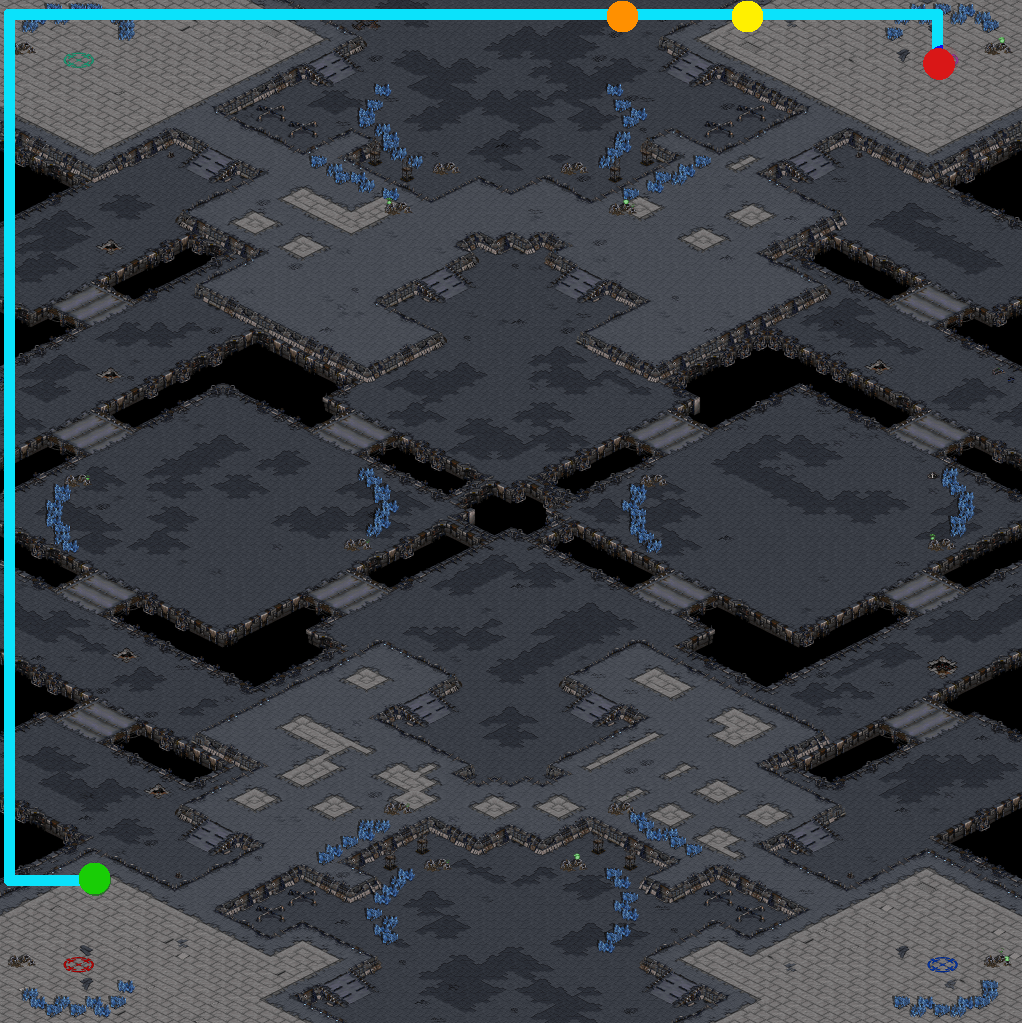
\includegraphics[width=0.75\textwidth]{space_atoll_(co-op)_drop_path}
\caption[Drop squad movement example]{Example of drop squad movement.
\usebox{\LegendDotGreen}~Start location where the transportation loads the units.
\usebox{\LegendLineCyan}~Path to the drop target.
\usebox{\LegendDotOrange}Squad waits here, if it has wait goals.
\usebox{\LegendDotYellow}Where the squad starts to unload.
\usebox{\LegendDotRed}Target location to attack.}
\label{fig:drop_squad_movement}
\end{figure}

\subsection{Patrol squad}
\label{sec:patrol_squad}
Patrols units between a set of locations, in the current version of BATS it only patrols between our defend positions which the \nameref{sec:defense_manager} takes care of. The units in the squad automatically attacks close enemies, but all units will not go to that location; instead another manager needs to tell the defensive squad what to do, e.g. the defense manager will tell the squad where to defend. The squad will move to the defended area and attack all units within the defend perimeter (\squadDefendDefendPerimeter), but will remain in the defended area until no enemy units are within the enemy offensive perimeter (\squadDefendEnemyOffensivePerimeter).

The patrol squad will never succeed with its goal, as the goal is to patrol between the specified locations the entire game— although the locations usually change during the game.

\subsection{Hold squad}
\label{sec:hold_squad}
The hold squad has one goal, to hold a location from enemies; any location could be held, but it is designed to hold choke points. The squad contains a hold location and a roam location. The hold location works in more or less the same way as patrol squad's defense location, i.e. if enemy units enter the defend perimeter (\squadDefendDefendPerimeter~in radius) it will move and attack those units, as the squad always will defend here it does not bother checking if enemies are within the enemy offensive perimeter as the patrol squad does. The roam perimeter (\squadDefendRoamPerimeter~in radius) is where the units in the squad will move to and stay until enemy units move within the defensive perimeter.

Terran siege tanks have a special ability when their are in this squad and the bot has researched the siege mode ability. The siege tank will automatically siege up in the roaming area effectively defending the hold perimeter (and other close positions) from its location.

Hold squads use \nameref{sec:unit_composition}s to know which units should be in the hold squad—section \ref{sec:unit_composition} describes unit compositions in general and listing \ref{lst:unit_comp_defend} shows the composition file used for hold squads. The current unit compositions used by BATS are listed below; the top is the composition with least priority, whereas the bottom is the one with highest priority. The name of the composition is in bold text.

\begin{function_description}
	\item[Marine spotter] 1 Marine
	\item[Bunker Marines] 4 Marines
	\item[Marine Medics] 4 Marines, 1 Medic
	\item[Tanks 1] 1 Siege tank
	\item[Tanks 2] 2 Siege tanks
	\item[Tanks 4] 4 Siege tanks
\end{function_description}
The Marine spotter is used to watch for enemies as one marine alone is not a good defender. Bunker marines are used for bunker, this strategy does not work with the current version of BATS as one cannot bind a hold squad to a specific location where there for example is a bunker. Marines and medics generally make a good composition, but these number are too low to hold of almost any attack, but they can still delay the attack until reinforcements can arrive, these are however not used in the experiment as none of the build orders build medics. Tanks are very good positional holders and can hold of almost anything coming through choke points\cite{day9}.

\subsection{Scout squad}
\label{sec:scout_squad}
Scouts regions and expansions that have not been scouted for a long time, to be exact it will always move to the region or expansion that our team visited the longest time ago. The \nameref{sec:exploration_manager} handles this and thus the scout squad gets it target location from it. To avoid multiple scouts moving to the same location the scout location will set its last visit time when the squad gets the location, although it hasn't been visited at all.

When an enemy is seen close to the scout it will abandon its current scout location and find another one, the idea is to save the scout from being killed by the enemy. This, however, does not work correctly all times as the units will move away from the enemy and at the same time towards the goal, but if the new scout location happens to be on the other side of enemy the scout will just roam around the outer edge of the enemy. To be sure that the scout does not switch scout locations all the time when an enemy is present it will only switch once its close to any enemy, it will then need to get out of the range before it can switch goal again.

\paragraph{Further optimizations}
When another unit visits the target location the squad will not complete its goal until it has reached there itself. Currently the squad moves from one end of the map to the other (already passing recently scouted areas), an improvement would be to either let the squad get regions and expansions that abut to its current location (or more correctly improve Exploration Manager), or search for the most optimal path (in regard to visit not-recently visited locations) when moving to the target location—i.e. use its via path. The first option is probably preferable as it is easy to calculate and easy to check if the first limitation should be solved, otherwise one must check all via paths and the path might not be the optimal anymore if one location is removed.

\subsection{Unit composition}
\label{sec:unit_composition}
In a nutshell, the unit composition is a feature for the squads to require specific types of units. E.g. hold squads require specific unit groups (compositions) as was explained above in section \ref{sec:hold_squad}. All unit compositions used in bats can be seen in appendix \ref{sec:unit_compositons_in_bats}. The unit composition has two important elements: The priority and the units, higher value means higher priority, the units for the composition are listed under the units sub-section.

To use compositions one calls the unit composition factory which takes a composition type (hold-squad, drop, etc.) of and a list of units (usually free units). The unit composition factory will check which compositions can be created with the available units—the composition needs to be full—and then return these sorted by priority. It is then up to the caller of unit composition factory to decide which composition to use—for hold squads it will always use the one with highest priority, drops on the other hand takes a random one.

\subsection{Wait goals}
\label{sec:wait_goals}
Wait goals were created for simple one time trigger abilities. These can be added to any squad at the moment, but will only have an effect on the squad if the derived squad handles them, as the squad base class only checks if the wait goal has succeeded, failed, or timed out and send an event to the derived class.

To be updated wait goals shall be added to the wait goal manager which updates the goals, completed goals (succeeded, failed, timed out) will automatically be removed from the wait goal manager. When adding an wait goal to the manager an optional set type can be set, this allows all wait goals with the same set type to be easily extracted—\nameref{sec:attack_coordinator} uses this when adding existing wait goals to a new attack squad.

\paragraph{Existing wait goals}
For now there is only one type of wait goal, WaitReadySquad. \nameref{sec:attack_squad}s uses these, as described in section \ref{sec:attack_squad}, to synchronize all its attacks—i.e. to attack the enemy simultaneously from different locations. The wait goal will complete when the attack squad is in position, \squadAttackWaitingPositionDistanceFromGoal from the attack location, when the squad is under attack or attacks, or if the wait goal times out (\attackCoordinatorWaitGoalTimeout).

% !TEX root = ../../main.tex
\section{Build planner}
% !TEX root = ../../main.tex
% !TEX spellcheck = en_US 
\section{Communication}
\label{sec:communication}
BATS uses the IntentionWriter to send messages to the teammate, a message consists of an
intention together with an optional reason and ping location.
Each intention and reason has multiple messages and are picked at random and put together to form a 
sentence with the intention first—if no reason is specified it will only use the intention as
the whole message. The random function, however, is not entirely random, it will never pick the last
used intention or reason message.

To not spam the teammate, messages with the same intention share a timeout, default set to 30\conf~in-game
seconds; if the bot tries to send another message with the same intention before it has timed out
IntentionWriter will skip the message. The timeout can be overridden by each intention, for example
warning that BATS is under attack has a timeout of 60\conf~in-game seconds.

All messages and timeout settings are read from an ini-file to easily add, change, or remove
existing messages, and to reload messages during gameplay. See appendix
\ref{sec:intention_and_reason_messages} for the full ini-file with all intention and reason
messages.

This simple communication system that picks two parts of the sentence at random and put them
together works relatively well. A better approach would be to create
specific messages for each intention and reason together, i.e. not randomize one from intention
and one from reason, but create around 5 messages for each combination. This will create more
tailored messages and will have better English, as this system has some limitations (described
below). This was not implemented because it required much more sentences and thus time.

\paragraph{Limitations}
Because the intention message could be used with many reasons the intention needs to be generic and
cannot be tailored to the situation. E.g. ``Falling back'', ``I'm retreating'', instead of ``Fleeing
from the enemy'', while all work for the reason ``because the enemy is too strong'' the last
intention will not work for ``because you're retreating.''

Many of the sentences may sound a bit strange and some could sound auto-generated. For example ``I
will attack, you're expanding'' and ``Leeeerooooooooy Jenkins, because I'm
expanding''\footnote{Leroy Jenkins is an Internet joke from World of WarCraft where Leroy was tired
of waiting of his group and ran into several mobs (monsters) killing the entire group. In the
beginning he yelled his name, thus this message.}, but maybe not ``I will attack, while you are
expanding'' or ``Sending out an attack, because I'm going to expand.''

% !TEX root = ../../main.tex
% !TEX spellcheck = en_US
\section{Evaluation and experimentation methods}
To evaluate our bot (and later our hypothesis) we conducted three evaluations and a final experimentation. The first evaluation was in the design phase of the bot. Here we asked StarCraft players on forums\footnote{
Team Liquid: \url{http://www.teamliquid.net/forum/viewmessage.php?topic_id=308630}\\
Battle.net: \url{http://eu.battle.net/sc2/en/forum/topic/3312961916} accessed 2012-09-03.} what they would like to see in a teammate bot.
%: Write about what features they would like to see.
\marginpar{write about features}

Close to when BATS was finished the authors played with it find remaining bugs and minor improvements that could be made. When the majority of the bugs was fixed, an additional tester evaluated the bot’s control and behavior to find further improvements that were needed before the final experiment.

\paragraph{Player evaluation}
From the player evaluation we conducted that an improvement needed to be made to how commands were send. For one available commands weren’t visible to the player, but s/he had to remember them. This gave the idea to create GUI buttons for the player client. These can be seen in figure \ref{fig:player_commands_gui}

\begin{figure}[htb]
\centering
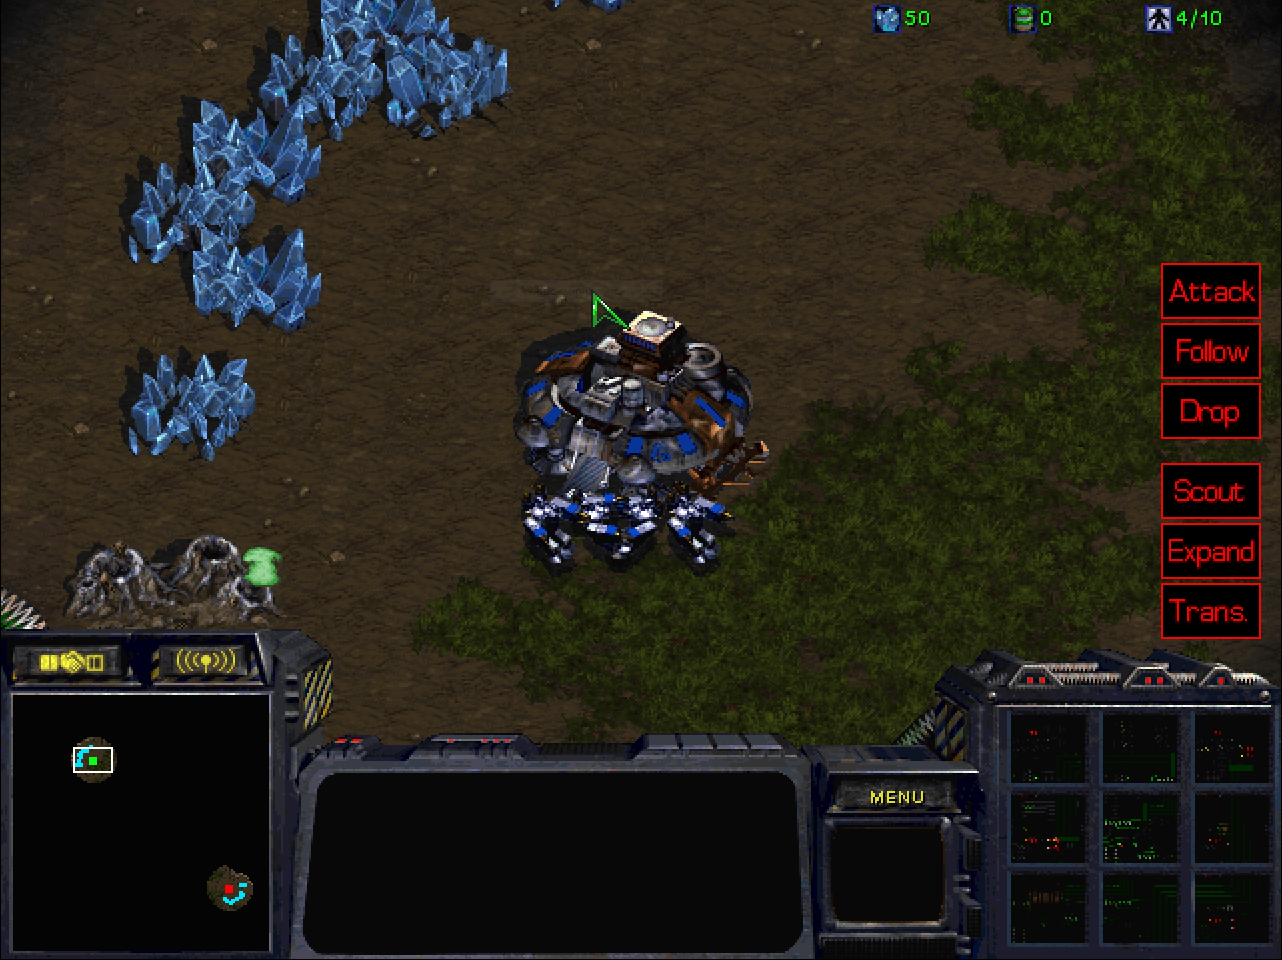
\includegraphics[width=0.8\textwidth]{player_gui_controls}
\caption{Player client with GUI commands enabled}
\label{fig:player_commands_gui}
\end{figure}

\subsection{Experiment method}
The experiment is divided in three parts, first the player preparation where the player would play skirmish matches against the default AI to refresh his/her skills or familiarize him-/herself with StarCraft and the map, the experiment will be conducted on. This could be done a couple of days before the experiment to the same day the experiment was, depending on the tester’s preferences.

The second part was the actually experiment itself. Here the player was presented with four scenarios he would play.
\begin{inparaenum}[1\upshape)]
	\item No control over the bot and the bot would not communicate its intentions;
	\item With control over bot, but no communication;
	\item With communication, but no control; and
	\item With both control and communication enabled.
\end{inparaenum}
To \h1{avoid a scenario preference depending} on the orders, the testers will use a different ordering of the scenarios. This will, however, have a side effect: Tester that start with both communication and control might be overwhelmed with both having a teammate and the need to check it’s intention messages and be able to control it.

The scenarios are played at fastest game speed, both because normal speed is slow (the experiment would be too long) and it is considered a standard to play at fastest game speed in the StarCraft community, although the campaign is played at normal game speed. Each scenario had a limit to 20 minutes because the testers could otherwise have played hour-long scenarios. If the player is winning after 20 minutes, the tester was asked if we should speed up the game or close it—the matches were sped up to roughly 10 times faster speed (depending on computer speed), thus the game usually ended within a minute or two. This was done to let the player win for the experiment to continue to be interesting.


% !TEX root = ../main.tex
% !TEX spellcheck = en_US
\chapter{Results}
These are the results from testing the bot on 14 people, 12 males and 2 females, ages 21–26, with skills varying from beginners who only had played StarCraft few times to those who have played more than 20 hours skirmishes in either StarCraft: Brood War or StarCraft 2.

\subsection{RQ 1 Which type of bot is most fun to play with?}
``Which is most fun to play with, communicating bot, controllable bot, both communicating and controllable bot, or none?''
Figure \ref{fig:results_fun} shows the questionnaire results from the four questions, one for each scenario. It was interesting that there also existed people who preferred only communication over both control and communication. In addition we saw a correlation between player skill and control preference from the interviews. Players with higher skill wanted the control feature whereas players with lower skill did not want or use the control feature.

\begin{figure}[htb]
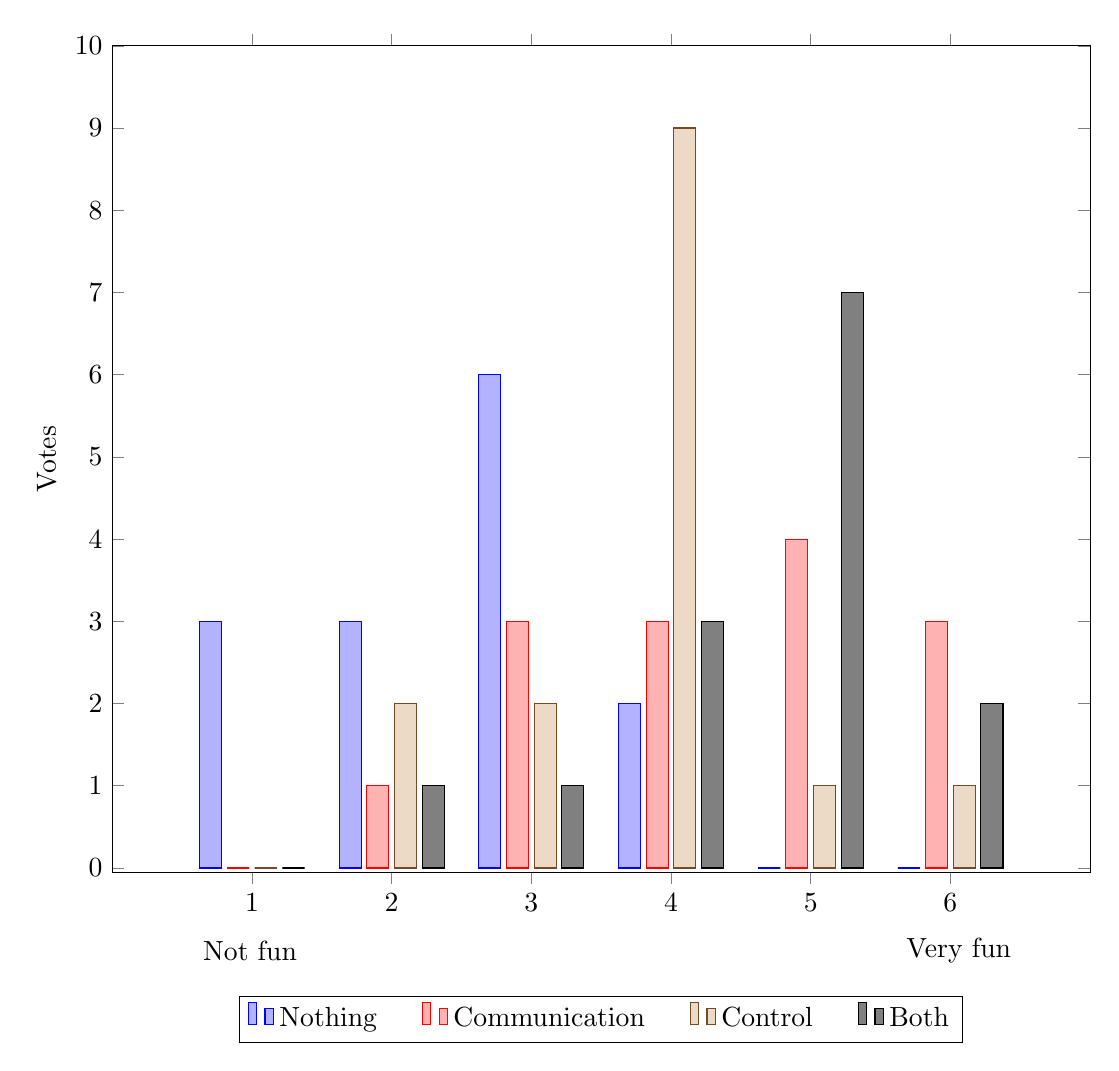
\begin{tikzpicture}
\begin{axis}[width=14cm,
	ylabel=Votes,
	ymin=-0.05,ymax=10,
	xmin=0,xmax=7,
	enlargelimits=false,
	xtick=data,
	legend style={at={(0.5, -0.15)},
		anchor=north, legend columns=-1,/tikz/every even column/.append style={column sep=0.5cm}},
	ybar,
	bar width=8pt,
]

% no control, no communication
\addplot
	coordinates {(1,3) (2,3) (3,6) (4,2) (5,0) (6,0)};

% no control, with communication
\addplot
	coordinates {(1,0) (2,1) (3,3) (4,3) (5,4) (6,3)};

% with control, no communication
\addplot
	coordinates {(1,0) (2,2) (3,2) (4,9) (5,1) (6,1)};

% with control, with communication
\addplot
	coordinates {(1,0) (2,1) (3,1) (4,3) (5,7) (6,2)};

\legend{Nothing, Communication, Control, Both};
\end{axis}
\node at (1.75,-1) {Not fun};
\node at (10.75,-1) {Very fun};
\end{tikzpicture}
\caption{Fun degree of the four scenarios}
\label{fig:results_fun}
\end{figure}

\paragraph{Control \& communication}
During the interviews 8 of 14 testers felt it was most fun to play with the bot when it had both communication and control on. Two of the tester could not decide whether only communication or both communication and control was more fun, but one mentioned that s/he would liked control and communication more than only communication if s/he had been better at the game. Testers' reasons why this scenario was most fun to play.
\begin{itemize}
	\item Build up my army and order he to attack and attack with him.
	\item Easier to plan because he told me his plans.
	\item I could order him to attack where I attacked using the follow command.
	\item You get a direct response from him after an order—you know that something will happen.
	\item Nice to be able to control him.
	\item Fun to see which strategies he uses.
\end{itemize}

\paragraph{Communication only}
6 of 14 testers (including the two testers already mentioned that could not decide on whether only communicaiton or both communicaiton and control was most fun) thought it was most fun to play with the bot when it only had communication on. Testers' reasons why this scenario was most fun to play.
\begin{itemize}
	\item I already had a lot on my mind, controlling him was a bit too much for me.	
	\item Easier to plan because he told me his plans.
	\item I am lazy therefore it was easier to let the bot do its job.
\end{itemize}

\paragraph{Control only}
2 of 14 testers thought it was most fun to play only with control. Although these might not be credible as for one tester it was the only game s/he won in the test and s/he told us that it was only because of that it was most fun, otherwise s/he guessed it would be more fun with communication. The other tester only thought control was most fun as it was the first scenario s/he tested, otherwise s/he thought control and communication was most fun because it was easier to play when I (the tester) can send attacks at the same time his and it gets easier to see what the bot does, i.e. same reasons as other players who thought control and communication was most fun.

\subsection{RQ 1.1 Which features are most liked?}
Below the most liked features are shown in two lists, one containing general features and the other specific commands they liked. Features mentioned by at least half (6) of the testers are marked as \textbf{bold}.
\paragraph{General liked features}
\begin{itemize}
	\item \textbf{Communication}
	\begin{itemize}
		\item He said why attacked, expanded, and so forth—I could learn from his strategies.
		\item \textbf{Fun to know what the bot is doing.}
		\item \textbf{Easier to plan because he told me his plans.}
		\item Feels more like team play when he is communicating.
		\item Direct response after ordering a command, then you knew if the bot would follow the command or not.
		\item It had humor, e.g. Leeeeroooooooy Jenkins.
		\item Almost like playing with a real player.
		\item Asked player for help when under attack.
	\end{itemize}
	\item Uses strategies that people uses, such as attacking when expanding.
	\item Very good macro.
	\item Own initiative to do things.
	\begin{itemize}
		\item Followed me when I wanted to attack, even though I did not order him—feeling that I play with someone.
		\item Very good at expanding, and often.
		\item I could act after how it acted and collaborate.
	\end{itemize}
	\item Coordinated defense—came and defended me when I needed help.
	\item It did not run its own race, I felt more involved in its decisions.
	\item Built tanks—I could back with my units and the tanks would clear the enemy units.
	\item Its attack cleared the path for me.
\end{itemize}

\paragraph{Liked commands}
\begin{itemize}
	\item Follow
	\begin{itemize}
		\item Doubles the amount of army size at one place.
		\item I do not like attacking by myself which the follow command explicitly prevented.
		\item Easier to coordinate where he should attack.
	\end{itemize}
	\item Attack
	\begin{itemize}
		\item I do not have to move there with my own troops.
		\item He could clear the path for me.
		\item Easy to reinforce as one could spam the attack button.
		\item He always had an army, if he attacked I could support him with my smaller army.
		\item He decided where to attack and I could follow and attack somewhere close.
	\end{itemize}
	\item Expand
	\begin{itemize}
		\item I control the timing between when I attacked and he expanded.
		\item I could order him to expand twice if the opportunity came, or just to expand when he did not notice he could expand.
	\end{itemize}
	\item Scout
	\begin{itemize}
		\item I do not have to scout and that is good as I am lazy.
	\end{itemize}
\end{itemize}

\subsection{RQ 1.2 Which features are most disliked?}
Instead of asking what features the testers disliked, we asked what they disliked about BATS (notice the removal of feature). Below is a list of all things they disliked about BATS. Common dislikes mentioned by at least half (6) of the testers are marked as \textbf{bold}.
\paragraph{General disliked features}
\begin{itemize}
	\item \textbf{The army halted in choke points and made it impossible for me to come through.}
	\item Got stuck when moving to a place, he ran back and forth until he finally ran more too long to the other side—note: grouping behavior.
	\item It did not follow me very well—note: when the squad it followed became very small (1-2 units) the player did not notice it had units that the bot followed with 30+ units.
	\item Bot asks for help when few units attack and he can easily handle it.
	\item Felt like it changed how good it was during each scenarios.
	\item He attacked cowardly, slow attack with siege tanks instead of just marching in and killing everything which he could do in most situations.
	\item Sends to many messages at the same time, maybe queue up messages instead?—note: sometimes the bot will decide to retreat, but then it decides to attack directly after and then expand because it is attacking, thus 3 messages are printed directly after each other which can confuse the player as it did in some cases.
	\item Never had units for drops.
	\item When it dropped it did not function very well.
	\item A better scout that scouted bases and not random locations.
\end{itemize}

\paragraph{Disliked commands}Two answered drop as it did not work properly, but most of the testers did not test all commands and thus could not answer if they disliked any command.

\subsection{RQ 1.3 Which features are missing?}
The testers were asked which features they missed during their scenarios, the first list presented includes general features whereas the second list are specific commands they missed.
\paragraph{General missed features}
\begin{itemize}
	\item More strategies, e.g. rush attacks, and would know about timings to make use of them.
	\item Use a variety of strategies depending on my build order.
	\item Give resources to the bot.
	\item Did not specify where he is under attack, would help me find the place.
	\item BATS could communicate what it think the player should do when s/he does not now what to do.
	\item More variety of units, more detection units.
	\item Scans in enemy base.
	\item For the bot to play other races than Terran.
\end{itemize}

\paragraph{Missed commands, or improved existing commands}
\begin{itemize}
	\item A help button when the bot shall come and help me.
	\item Using way points for attacks to direct from where he should attack so he did either did not block my path or to create a more advanced attack.
	\item Drunken mode, random behavior.
	\item Command buttons grayed out when player could not use them.
	\item Retreat command.
	\item Abort command to abort the last command if the player misclicked.
	\item Hold position.
\end{itemize}

\subsection{Other questions and comments}
\paragraph{What surprised you in a positive way?}
A common misconception was that the testers would play against the bot and not with it. They thought BATS was a good bot, that built up his army fast and that the tester did not need to babysit it. They tended to like the funny messages, especially Leeeeeerrooooooy Jenkins. Common for many testers were that the bot expanded just before they were going to send the expand command, which made them think the bot was good at expanding and had a good timing on expands. A tester liked the underlying reason behind each intention and not just the intention as s/he could learn from this. Another tester was surprised by that it worked so well to play with a bot as they can be quite stupid.

\paragraph{What surprised you in a negative way?}
More than half of the testers thought BATS crowded the places he attacked and made it impossible to bypass unless you had air units, 2 testers even changed their strategy to only air units because of this. He did not clear the entire base as humans would do, but left the base when few buildings were left. Twice the bot expanded to a location the player already expanded to, i.e. build a command center beside their command center (or equal building). Sometimes the bot followed a small army consisting of 1-2 units, this surprised the player as s/he it would either retreat or continue attacking on its own.

\paragraph{If you won or lost, did you think it was because of the you, BATS, or both?}
This question was not asked until the 6th tester, thus only half the testers were asked this question. Three of the tester thought they won because of both, where one of these thought it was because of him/her in one of the four scenarios. Their reasons were that BATS was better at building units, but they themselves had a better idea of strategy, where and how to attack. Two of the testers thought it always because of them as they felt better than BATS, these two were amongst the better players and also preferred control—a side note, there were two other players just as good as them, one of them thought it was because of both and strangely the other thought it was because of the bot.

There were only one loss for the last 6 tester. The tester who lost felt that it was entirely his/her fault as the bot had been attacked for 4 minutes and was defeated before the tester even noticed it, although s/he mentioned that if the bot had said it was under attack it would never have happened.

\paragraph{Commands used}
We noticed that many of the testers did not use all commands, no-one used the transition command as all felt the bot handled that fairly well. Only a few (2–4) used the drop, expand, and scout commands, with the same reason here as they felt the bot did a good job on this, except drop but they did not feel as a drop was needed.

\paragraph{Other noteworthy comments}
One tester mentioned the bot felt like Brother in Arms where you can control other units. Another tester mentioned that it was more fun to play with this bot than any other s/he had played with. A third tester thought BATS could be used either when one wanted to play a regular co-op game but did not have any friend to play with, or to fill an uneven team when playing with friends.

\subsection{Questions and comments about the experiment}
These are questions asked about the experiment itself and not directly associated with the bot.

\paragraph{Was the experiment fun or boring, and why?}
All testers thought it was fun to test the bot, both because StarCraft is a fun game and because it was a new experience for many to play with a bot that you could control and communicate.

\paragraph{Was the experiment too long?}
The experiment was estimated to take 2 hours. Some testers thought it sounded quite long, but none of the testers thought it was too long. Their reasons were that the scenarios were short (max 20 minutes) and they had fun testing the bot making time pass very quickly.

\paragraph{Other comments}
A tester commented how much difference there were between bots with and without communication, put in the testers own words: ``I noticed how important the communication was and how bad something can be when a feature is missing.''\footnote{Translated from Swedish ``Jag märkte hur viktig kommunikationen var och hur dåligt någonting kan vara utan en feature''}
% !TEX root = ../main.tex
\chapter{Related work}
% !TEX root = ../main.tex
% !TEX spellcheck = en_US
\chapter{Conclusions and future work}
First we go through our conclusions on the bot, what the players thought, liked and disliked about
the bot and scenarios. Then we go through some lessons we have learned during the project we thought
was worth mentioning, and last future work for researchers where we focus on three different areas:
teammate bot behavior, communication, and control.

\section{Bot conclusions}
We conclude that a teammate bot for RTS games that communicates its intentions and reasons is indeed
more fun to play with, although we did not find any statistical difference between Communication +
Control and only Communication both of these include communication.

What surprised us was that some players
preferred when the bot only communicated. This was later identified to depend on the player's skill
where more experienced players liked the ability to control the bot whereas beginners tended to get
overwhelmed by all the existing game action and thus did not want to focus on yet another task:
controlling the bot. This is an interesting question on how to balance the control so that
beginners aren't overwhelmed but at the same time meets the needs of a more skillful player. We talk
more about this below in section \ref{sec:future_control}.\\


The most liked feature was the ability for the bot to communicate its intentions and reasons to the
player. The most reasons were ``it was fun to know what the bot is doing'' and ``easier to plan
because he told me his plans''. This aligns with what Norman states, humans want to know what the AI
is doing\cite{norman07}.

An important aspect BATS missed was point 5 from McGee's and Abraham's definition\cite{mcgee10} of a
real-time teammate bot, ``whenever possible, prioritizing the player experience''—for the full list
see section \ref{sec:teammate_bots}. When the player either ordered BATS to attack or follow
him/her, BATS almost always ended up blocking the path for the player close to the attack location,
not prioritizing the player experience as it should let the player through.
Disrespecting this ``rule'' probably made ``The army halted in choke points and made it impossible
for me to come through'' the most disliked feature.

\section{Project conclusions}
\paragraph{Magnusson's notes}
Being a perfectionist is not easy, this was one of the causes why we did not meet our first
deadline. I implemented features that were never used but what I thought were nice to have, such as
the Wait Goals, advanced drop mechanics. If we remove Wait goals and drops entirely it would
probably not affect the test results as Wait goals were never used and drops were barely used.
In addition to this I changed existing systems much more than
needed—instead of using the existing squad manager with squads I create a new squad manager, this
was because the functionality differed quite much what we wanted to have in BATS, but maybe not
needed. We would have saved some weeks on this task alone.

In addition I tweaked and fixed small thing that ``it will only take two hours'', but I found many
of these small tweaks and some of them took more than two hours. After half the bot had been
implemented and the deadline was close, we decided to decrease the number of features and aim for
the next deadline, almost three months later. Now instead for fixing all small bugs and tweaks I
created a ticket in our project manager, then I forced myself to not work on them until all the
bot's main features were implemented. This worked much better and the bot was done, maybe not in no
time, but much faster.

In essence what I learned was that task prioritization is a must if one wants to finish a project,
and then only work on those assigned tasks, if new tasks were found one shall not do them directly
but either put them in the right priority or put them in a bag of things to do if there is time
left.

\section{Future work}
We will split the section in three parts, first discussing future work for the behavior of a
teammate bot, then improvements on the communication, and finally the control of a teammate bot.
While these are RTS game specific topics many of the Communication and Control topics can be
slightly changed to match another game genre.

\subsection{Teammate bot behavior}
BATS behaves in ways that we thought would be good, both through own experience, research, and
testing; but it still lacks a solid behavior to be used in a commercial game as its behavior does
not change depending on the play style of the human player. More research needs to be done on what
players want a teammate bot to do and how much initiative the bot shall have. If the bot can be
controlled the degree of initiative can depend on how much the player want to control the bot, i.e.
the more control the player wants the less initiative the bot shall have, or does the players,
independent of skill and play style, always want the same initiative?

A possibility for teammate bots can be either a full-time or temporarily replacement for a human
player in online matches—temporarily when the player disconnects. But how shall the bot behave when
it is used as a replacement for the entire game? It needs to be balanced so it either matches the
human players' skills in its own team or by setting a predefined skill to either increase or
decrease the entire team's total skill. When it acts as a temporarily replacement the players might
want it to continue using the same strategy as the player and not do any hasty actions that could
make the player loose, the bot could use some learning algorithm that always is on when the player
plays matches and then send out this information to the other clients if the player gets
disconnected, one of the clients could then take temporary control of the player continue play as
nothing happened.  For both scenarios it might be good to do player modeling for the teammate bot to
know how it shall play, further resources on player modeling for RTS games can be found
here\cite{bakkes09, jansen07, kabanza10, schadd07, synnaeve11}.

\subsection{Communication}
The messages from BATS are very simple and aimed to feel like less auto-generated messages. In case
of text messages the player might not want long ``human-like'' sentences, but instead short
sentences.

There is also the possibility to either synthesize the message or record own messages to see if the
player prefer messages that are read to him/her.  Reading messages out loud might be good but cannot
be processed as quickly by the player and it can be hard if the computer want to send messages very
often, meaning some research needs to be done on how often and what type of messages shall be sent
for the player not to be overwhelmed by messages—this type of research can also be done on text
messages.

\subsection{Control}
\label{sec:future_control}
We concluded that not all commands were used and players preferred control depending on their skill.
One could research which type of commands are preferred and how often they are issued. This could
then serve as another research where more control functionality is either displayed for a player
depending on his/her skill level, for example in campaigns the game introduces new units for each
mission and could in a similar way introduce more commands throughout the entire campaign.

Another experiment could be made how much level of detail the player wants over the commands. E.g.
shall attack make the bot attack at some place (as it does now), shall the player have the ability
to specify where it shall attack, shall the player have the ability to specify which path the attack
shall use, or where the attack shall wait before it reaches its destination for a simultaneous
attack?  This level of degree probably depends on the skill of the player, but as you might have
thought of now this can cause the player to simply play two players, but s/he only needs to control
one bot. This leads to yet another research for a new genre.

Research a new type of RTS genre where the player simply tell the bot what to do, i.e. the player
control the bot entirely but has setup some rules what it should build and how it behaves. This
would be more like a strategy/tactic game where the player neither needs good macro nor good micro, but
good strategy and tactics.

Mentioned in behavior, the possibility exists for acting as a player replacement in a team with more
than 2 players. In regard to control, who shall control the bot, or can anyone in the team control
the bot? Anytime?

% !TEX root = ../main.tex
\appendix
% !TEX root = ../../main.tex
% !TEX spellcheck = en_US
\chapter{Intention and reason messages}
\lstinputlisting[label={lst:messages},caption={Intention and reason messages ini-file},language=ini]{code/messages.ini}

%%  \include the `end matter'

%
% New style of Bibliography
% http://amath.colorado.edu/documentation/LaTeX/reference/faq/bibstyles.html
%
\bibliographystyle{plain}	% (uses file "IEEE.bst")
\bibliography{bibliography}
%
%\input{glossary}
%\input{index}
%\input{guide_symbols}
%\input{guide_curriculum}

%%  finally, \include the list of previous bth-CS dissertations

%\cleardoublepage % if you are so inclined
%\include{bthcsdissertations} %PERSONALIZE that is: make sure you have the
%latest list.
%\include{guide_back1} % for a thesis with a back-flap summary
\include{guide_back} %or take this one for a fairly plain back cover
 
\end{document}
